\documentclass{pnastwo}
\usepackage{cite}
\usepackage{color}
\usepackage{pgf}
%\usepackage{hyperref}
\usepackage[normalem]{ulem}
\newcommand{\jri}[1]{\textcolor{red}{\scriptsize #1}}
\newcommand{\citex}{\textcolor{red}{\bf CITE}}
\newcommand{\X}{\textcolor{red}{\bf X}}
\usepackage{multibib}

\begin{document}

\title{Demography and linked selection in wild and domesticated maize}
\author{Timothy M. Beissinger\affil{1}{Dept. of Plant Sciences, University of
    California, Davis, CA, USA}\affil{2}{US Department of Agriculture, Agricultural Research Service, Columbia, MO, USA}\affil{3}{Division of Plant Sciences, University of Missouri, Columbia, MO, USA} Li Wang\affil{4}{Iowa State University, Ames, IA, USA}, Kate Crosby\affil{1}{}, Arun
  Durvasula\affil{1}{}, Matthew Hufford\affil{4}{}, \and Jeffrey
  Ross-Ibarra\affil{1}{}\affil{5}{Genome Center and Center for population biology, University of
    California, Davis, CA, USA} }

\significancetext{Patterns of linked selection, or the impact of selection on sites that neighbor a functional variant, have been carefully evaluated in only a few species. \jri{not really. we need to rephrase here and cite the Corbett-Detig plos-bio paper somewhere -- they looked at a lot of species including maize!} In this work, we demonstrate that selection against deleterious mutations leaves a pronounced signature on the maize genome, reducing diversity in and immediately around genes. We show how demography interacts with selection to impact genome-wide patterns of diversity, including the important observation that rapid population expansion can increase the efficiency of selection as much as a sudden population bottleneck can weaken it. Along the way, we develop the first estimate the demographic parameters of the maize domestication from whole genome sequence data. }

\maketitle

\begin{article}

\begin{abstract}
  Unique selective and demographic operate on domesticated plant species. These forces interact during and after domestication to generate the patterns of DNA variability that are persistent in crop species today. To quantify the interplay between demography and selection, we investigated genetic diversity in maize, one of the most important crops for food, feed, and fuel world-wide. We utilized whole genome sequence data from 23 maize and 13 teosinte individuals to make inferences.  We obtained a complete estimate of the population size fluctuations and other demographic parameters experienced by maize as it was domesticated from teosinte. Here, we show that maize went through a domestication bottleneck with a population size of approximately 5\% that of teosinte before it experienced rapid population size expansion post-domestication. We observe that hard sweeps, specifically positive selection on new genic mutations, are not the primary force driving maize evolution. We find that a reduced population size during domestication decreased the efficiency of purifying selection to purge deleterious alleles from maize. However, expansion after domestication has since increased the efficiency of purifying selection to levels superior to those seen in teosinte. Our results demonstrate that in domesticated species, demographic and selective history in the ancient and recent past both contribute to genetic variability that is present today, providing substantial implications for the continued improvement of domesticated species.
  
\end{abstract}

\dropcap{D}omesticated plant species evolve in a unique fashion
compared to their wild counterparts \cite{doebley2006}. This
is a result of both the anthropomorphic nature of artificial selection on
domesticates \cite{purugganan2009} as well as the demographic characteristics of the domestication
bottleneck(s) that they tend to have experienced
\cite{ross2007}. However, the
complex interplay between selective pressures and demographic
limitations, and the impact that this interplay has on identifying
selection and understanding demography, is not fully understood. Although a large body of
research that involves searching the genomes of domesticated species for evidence
of positive selection exists \cite{hufford2012, he2011, vigouroux2002, chapman2008}, these studies tend to focus on
identifying or mapping particular genes or regions that play an
important role in phenotypic evolution. In contrast, knowledge regarding the impacts that demography and
selection have on whole-genome patterns of genetic variability remains limited.

For instance, supposed neutrally-evolving DNA is often used to estimate historical demographic
parameters of a population such as effective population size, structure, and expansion
history \cite{luikart2003, gutenkunst2009}. However, researchers have
called into question whether or not there are reasonable approaches
for identifying neutral regions of the genome, since the effects of
selection can be wide-ranging \cite{li2012, slotte2014}. For example, in
\emph{Drosophila} it appears that the majority of the genome is
impacted by the effects of selection through linkage
\cite{sella2009}. A natural next question, therefore, is how can
demographic parameters be estimated independently of
selective parameters? Human researchers have attempted to address this
problem by limiting analyses to only sites far from genes
\cite{gazave2014}, but as \emph{Drosophila} demonstrates, it is
difficult to be certain that sites even in gene-poor regions of the
genome are not influenced by linked selection. Ultimately, an understanding
of which sites have the potential to be adaptive, and how these affect
genome-wide patterns of variability through linkage, is required for
reasonable demographic inference.

Maize represents an excellent organism to study these
phenomena. Maize is a species of tremendous importance worldwide as
both a staple crop \cite{shiferaw2011} and as a model for
understanding plant evolution \cite{strable2009}. Broadly speaking, archaeological and genetic studies have
established that maize domestication is likely to have taken place in
 Mexico approximately 9,000 years bp
\cite{smith1995,matsuoka2002}. Teosinte, the most
recent wild ancestor to maize, remains extant throughout much of the
Americas \cite{wilkes1967}. Additionally, several large-effect
domestication loci \cite{doebley1995, wills2013, wang2015} and putative domestication
regions \cite{hufford2012} have been identified. But despite all that is
known about maize domestication, the parameters of the
domestication process remain uncertain. Specifically, the size of the
maize domestication bottleneck has not been estimated independently of
the bottleneck's duration, nor are there sequence-based estimates of the effective
population size of modern maize. Sequence information from maize and
teosinte plants may therefore be utilized to address these questions.

To that end, the objectives of our study were to 1) investigate the
relative importance of different forms of selection on whole-genome
variability in both maize and teosinte 2) research the impact that the
domestication process has had on genetic variability in maize, and how
this compares to the impact of a different demographic history in
teosinte; and 3) precisely estimate the parameters of the
maize domestication bottleneck. We show that our third objective, estimating the
parameters of domestication, is not possible without first completing
 objectives one and two, which demonstrate that as in humans \cite{gazave2014}, the
majority of maize non-genic DNA may reasonably be treated as
neutral. We achieve these objectives by utilizing
whole-genome-sequence information from 23 maize and 13 teosinte lines
sequenced as part of the Maize HapMap 2 panel \cite{chia2012}.


\section{Results}
\subsection{Patterns of diversity differ between genic and
  non-genic regions of the genome}
Our reanalysis of the maize HapMap 2 data \cite{chia2012} is consistent with earlier findings that patterns of diversity differ between genic and non-genic regions of the genome in both maize and teosinte \cite{hufford2012} (Figure \ref{fig:diversity}). 
In maize, mean pairwise diversity ($\pi$) within genes was significantly lower than at positions at least 5 kb away from genes (0.00668 vs 0.00691, $p<2\times 10^{-44}$). 
Diversity differences in teosinte are even more pronounced (0.0088 vs. 0.0115, $p\approx 0$). 
Differences were also apparent in the site frequency spectrum, with mean Tajima's D positive in genic regions in both maize (0.4) and teosinte (0.013) but negative outside of genes (-0.087 in maize and -0.25 in teosinte, $p<X$ for both comparisons).
These observations suggest that diversity in genes is not evolving neutrally, but instead reduced by the impacts of selection on linked sites. 

\begin{figure}
\centering
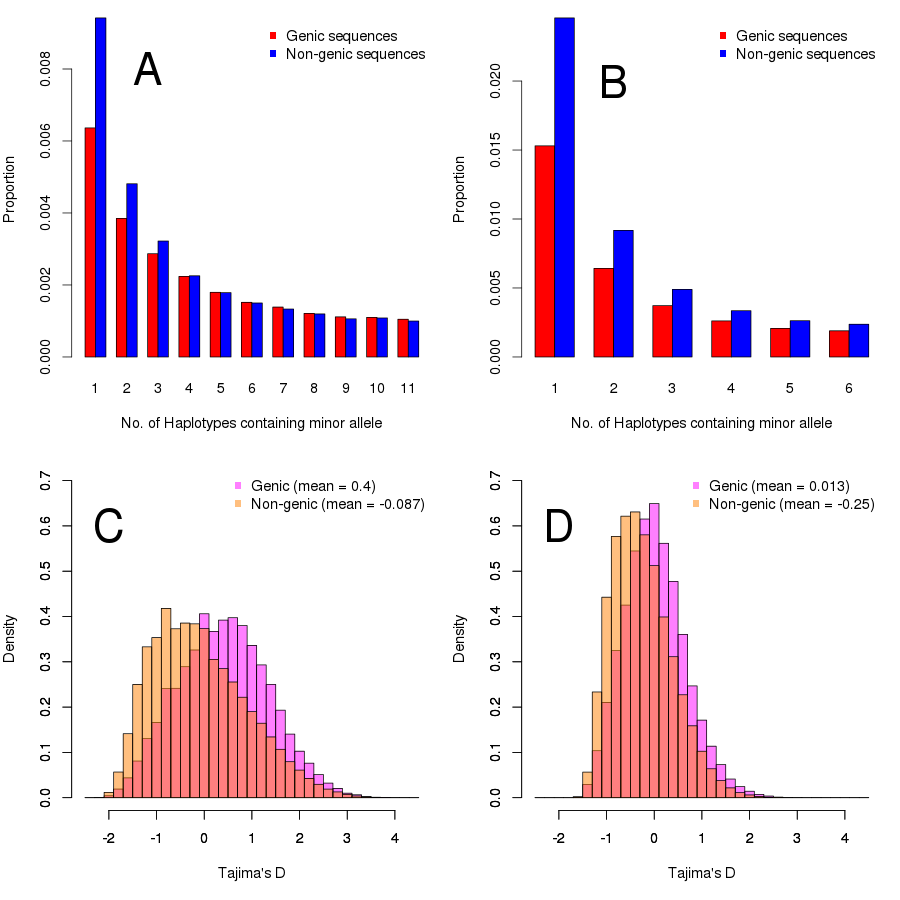
\includegraphics[width=.5\textwidth]{FigsAndFiles/SFS_and_Tajima.png}
\caption{The folded SFS and Tajimas D were calculated both inside and outside of genes for maize and teosinte. In both taxa, a dearth of rare alleles was observed within genes relative to outside of genes, which led to higher values of Tajima's D outside of genes than inside.{\bf A:} Folded SFS for maize; {\bf B:} Folded SFS for teosinte; {\bf C:} Maize Tajima's D; {\bf D:} Teosinte Tajima's D.  \label{fig:diversity} \jri{skip the SFS and make this a panel plot of pi and TajD in maize and teosinte} } 
\end{figure}

\subsection{Hard sweeps do not explain diversity differences}
Selection acting to increase the frequency of a new beneficial mutation will leave a signature of reduced diversity at surrounding linked sites \citex.
To evaluate whether patterns of such ``hard sweeps'' could explain observed differences in diversity between genic and non-genic regions of the genome, we compared diversity around missense and synonymous substitutions between \emph{Tripsacum} and either maize or teosinte (Figure
\ref{fig:hardSweeps}).
If a proportion of missense mutations have been fixed due to hard sweeps, diversity around these substitutions should be lower than around synonymous substitutions. 
We observe this pattern around the causative amino acid substitution in the the domestication locus \emph{tga1} (Figure \ref{sFig:tga1}), likely the result of a hard sweep during domestication \cite{wang2005origin, wang2015}.
Genome-wide, however, we observe no differences in diversity between synonymous and missense substitutions in either maize or teosinte.
Previous analyses in humans have suggested that this approach is limited by fact that a higher proportion of nonsynonymous substitutions will be found in genes under weak purifying selection and thus higher genetic diversity \cite{enard2014}. 
To address this concern we took advantage of a measure of evolutionary constraint using genomic evolutionary rate profile (GERP) scores \cite{davydov2010} calculated across the maize genome \cite{rodgers2015}. 
We re-analyzed substitutions in subsets of genes with the highest and lowest 10\% quantile of mean GERP score, putatively representing genes under the strongest and weakest purifying selection  (Figure \ref{sFig:consUncons}). 
As expected, we see higher overall diversity around substitutions in genes under weak purifying selection, but we still see no difference between synonymous and missense substitutions in either subset of the data.
Taken together, these data suggest hard sweeps do not play a major role in patterning genic diversity in either maize or teosinte.

%To ensure that this analysis is resilient to the intricacies of our sample, we investigated diversity surrounding the maize gene \emph{tga1}, one of the few known instances of a hard sweep corresponding to a causal missense substitution in maize \cite{wang2015}. In the case of this known sweep, we observed a reduction in diversity surrounding the causative substitution to levels much lower than seen for synonymous substitutions (Figure \ref{sFig:tga1}), confirming that this method should be informative if hard sweeps were the prevailing mode of selection in maize. 
%Still, to ensure that the approach is robust to potential shortcomings such as limited power in the face of background selection \cite{enard2014}, we sought to determine if patterns of diversity surrounding synonymous and non-synonymous substitutions differ when we restrict our analysis to the most- or least-conserved genes in maize. When we re-analyzed subsets of genes with the 10\% highest and 10\% lowest genomic evolutionary rate profile (GERP) score, putatively corresponding to genes undergoing the strongest and weakest purifying selection \cite{davydov2010, cooper2005, rodgers2015}, we again saw no significant difference in diversity surrounding synonymous and non-synonymous sites (Figure \ref{sFig:consUncons}).

\begin{figure*}[!htb]
%\vspace*{.05in}
\centering
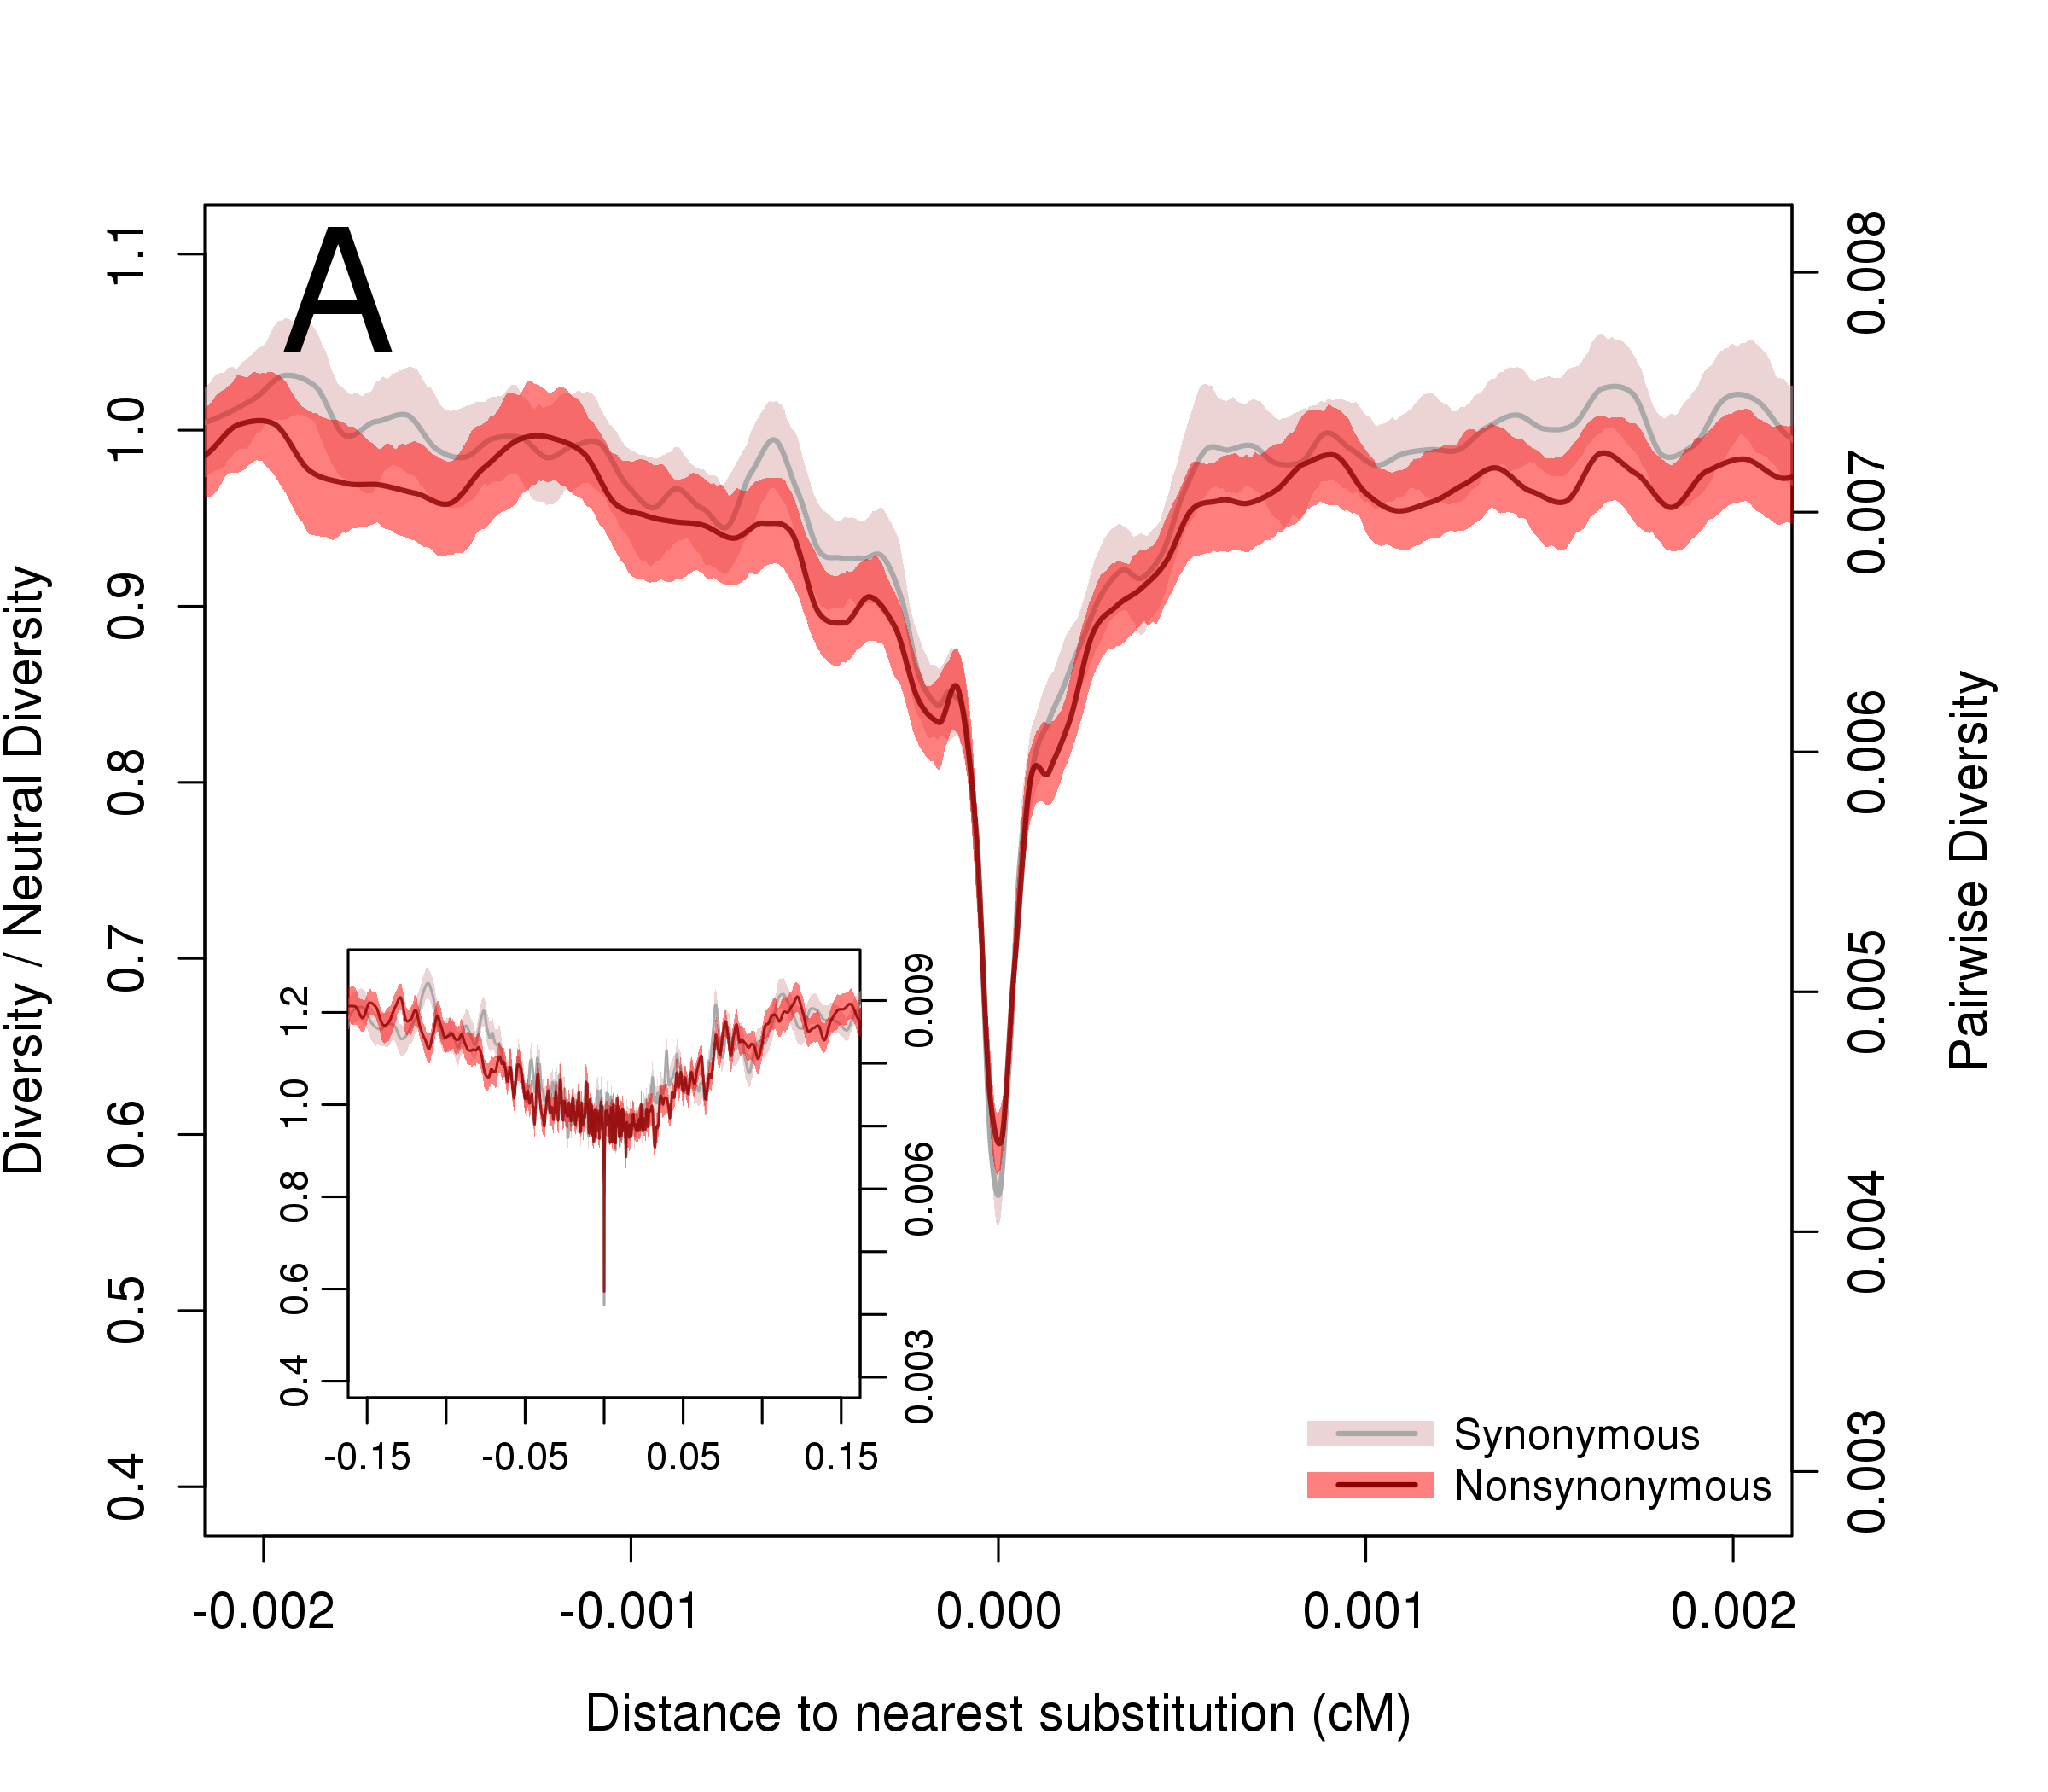
\includegraphics[width=.45\textwidth]{FigsAndFiles/plotDiversity_TvM_Folded2_Significance_Aug}
\hspace{0.05\textwidth} 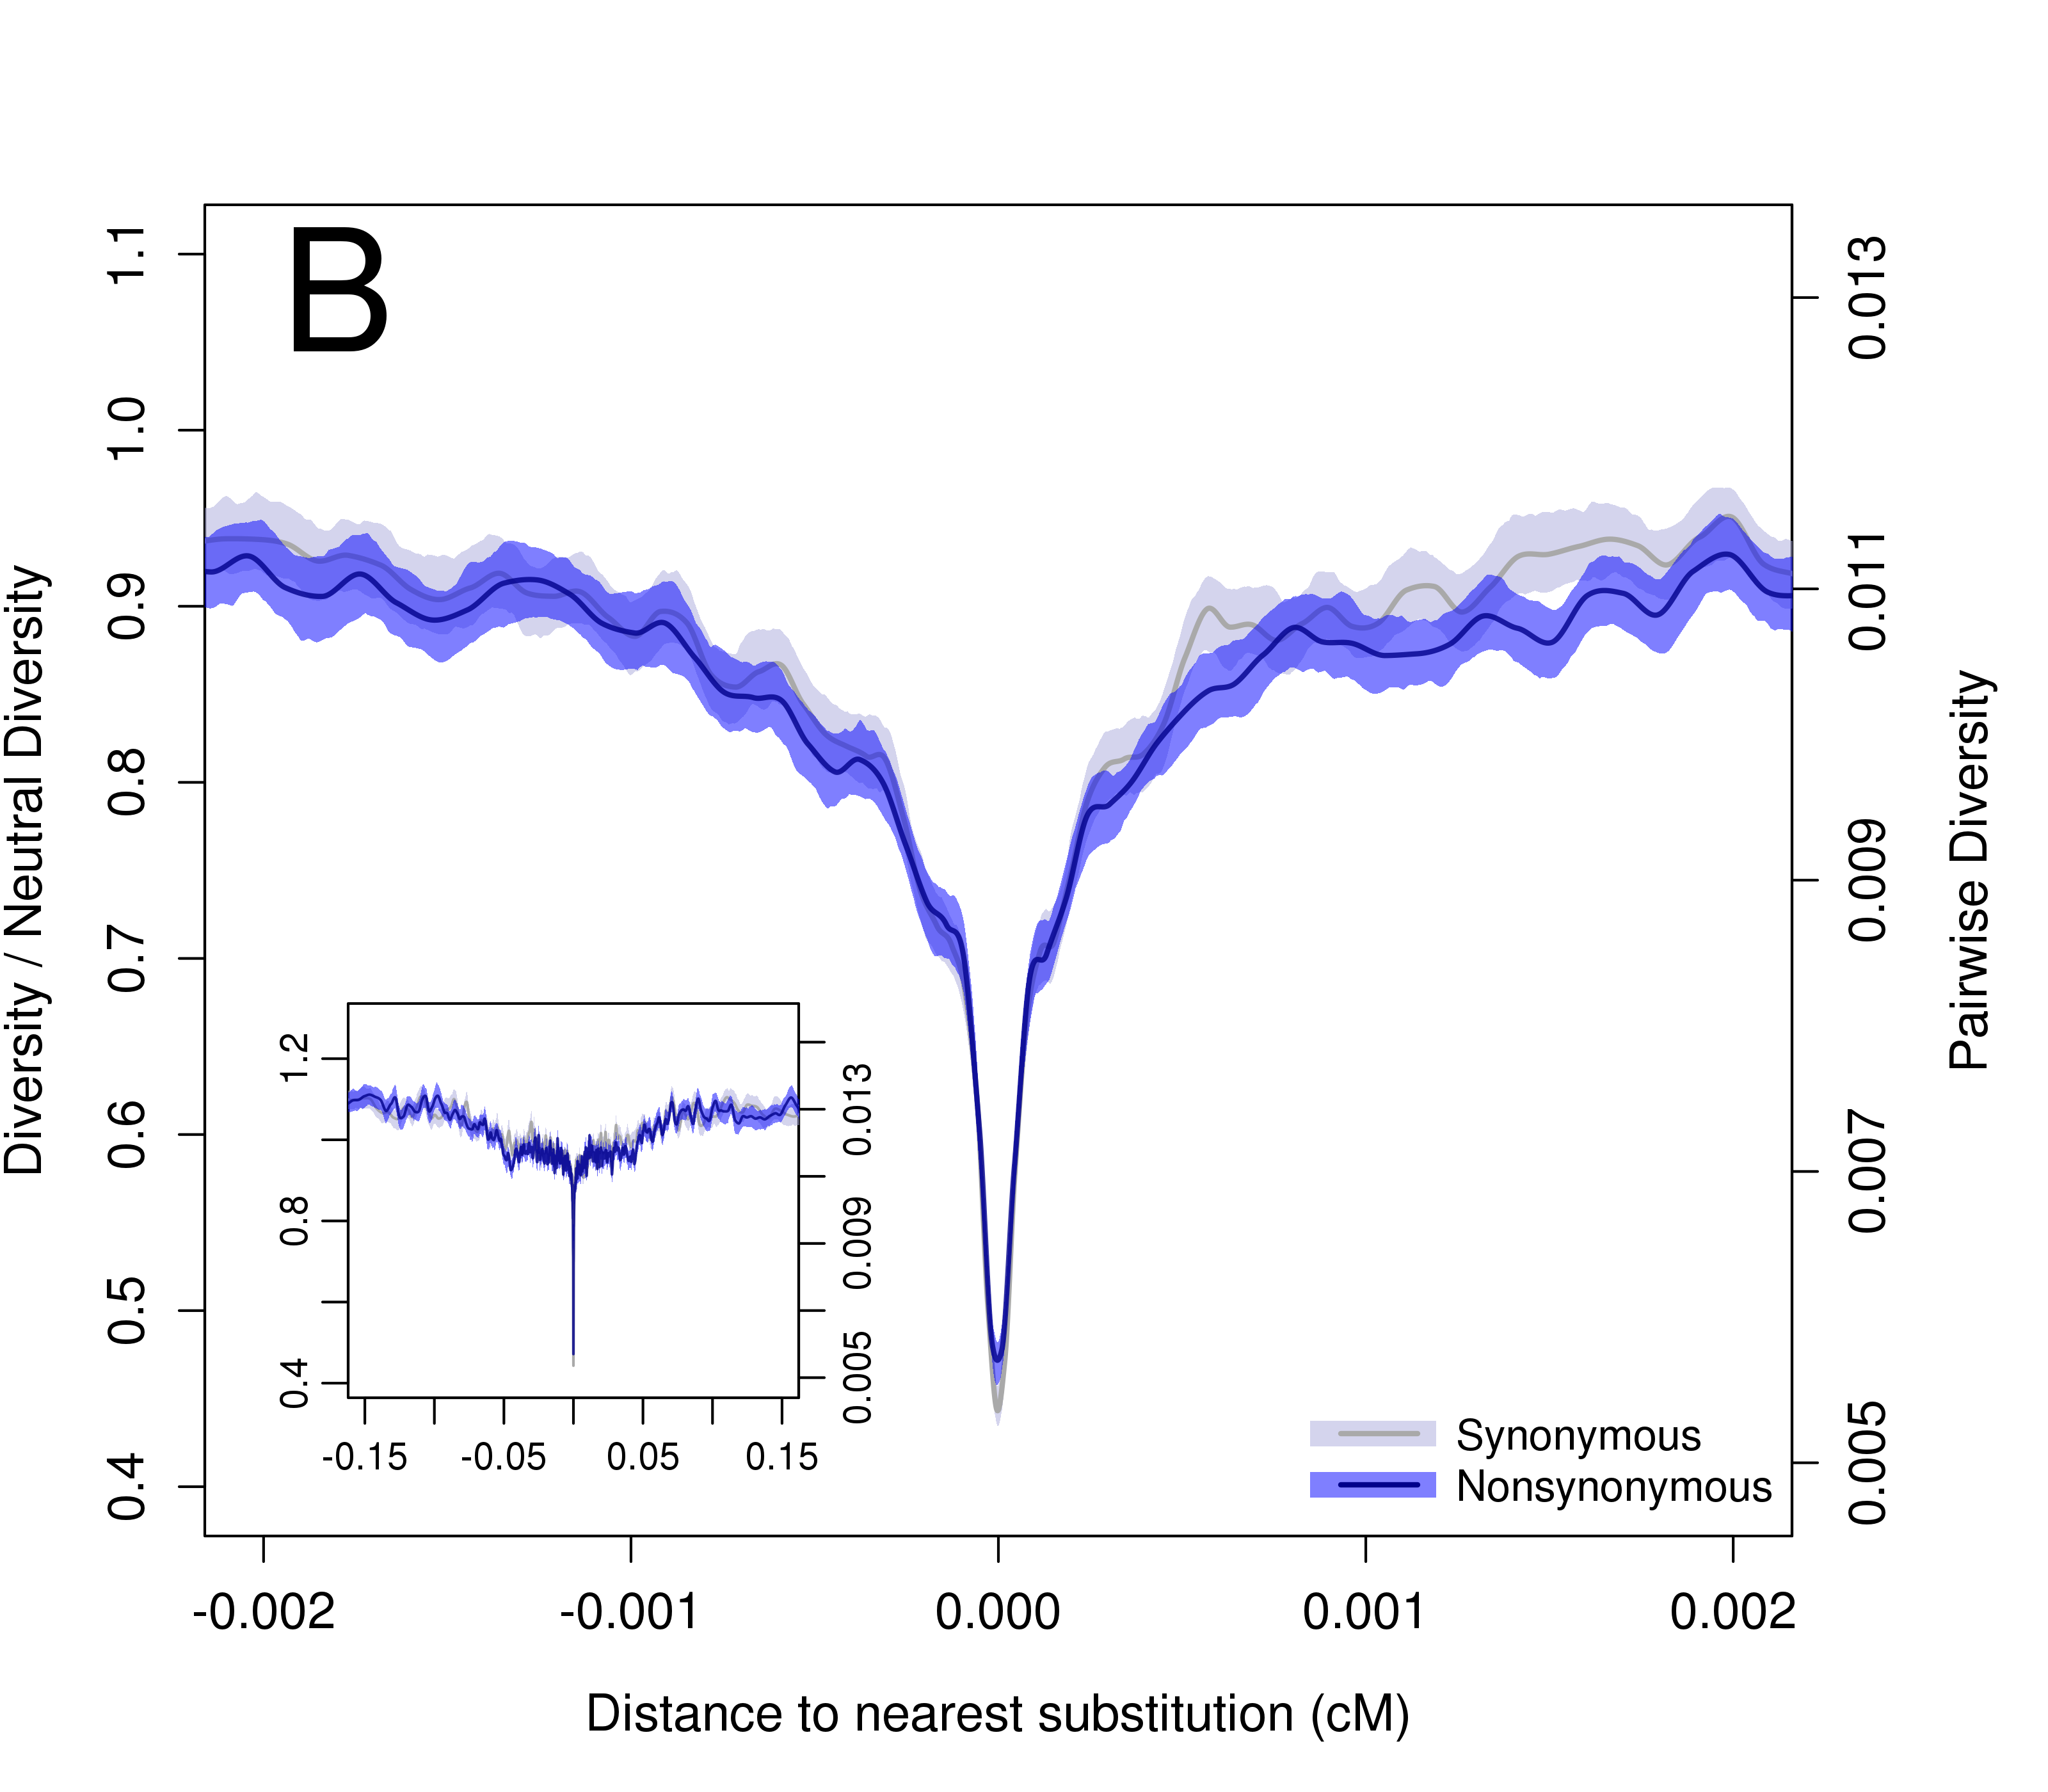
\includegraphics[width=.45\textwidth]{FigsAndFiles/plotDiversity_TvT_Folded2_Significance_Aug}
\caption{Pairwise diversity surrounding synonymous and non-synonymous
  substitutions in {\bf A} maize and {\bf B} teosinte. Axes show both absolute diversity values and values relative to mean nucleotide diversity in windows $\geq 0.01 cM$ from a substitution. \jri{is this correct or did i confuse things?}
 Lines depict a loess curve (span of 0.01)  and shading represents bootstrap-based 95\% confidence intervals. Inset plots depict a larger range on the x-axis. \label{fig:hardSweeps}}
\end{figure*}


\subsection{Pairwise diversity is heavily influenced by purifying selection}

Purifying selection refers to the situation where deleterious mutations arising in a population are continuously selected against.
When this form of selection is operating, it can serve to reduce genetic variability at linked neutral sites, a phenomenon often called background selection \cite{charlesworth1993}. Purifying and background selection lead to lower diversity within genes and other functional sites relative to neutral regions.
We investigated purifying selection in maize and teosinte by evaluating the average magnitude of reduced diversity within genes and recovery away from genes in both taxa.
To enable comparisons between maize and teosinte, we standardized by neutral levels within each taxa, where neutral levels were defined as mean diversity at positions at least 0.01 cM distal from genes. For both maize and teosinte, pairwise diversity was reduced within genes and a recovery of diversity away from genes was observed. Interestingly, a stronger reduction of diversity and slower recovery was observed for teosinte than for maize, implying that purifying selection has left a more pronounced signature on pairwise diversity in the teosinte genome (Figure \ref{fig:purify}).



\begin{figure*}[!htb]
%\vspace*{.05in}
\centering
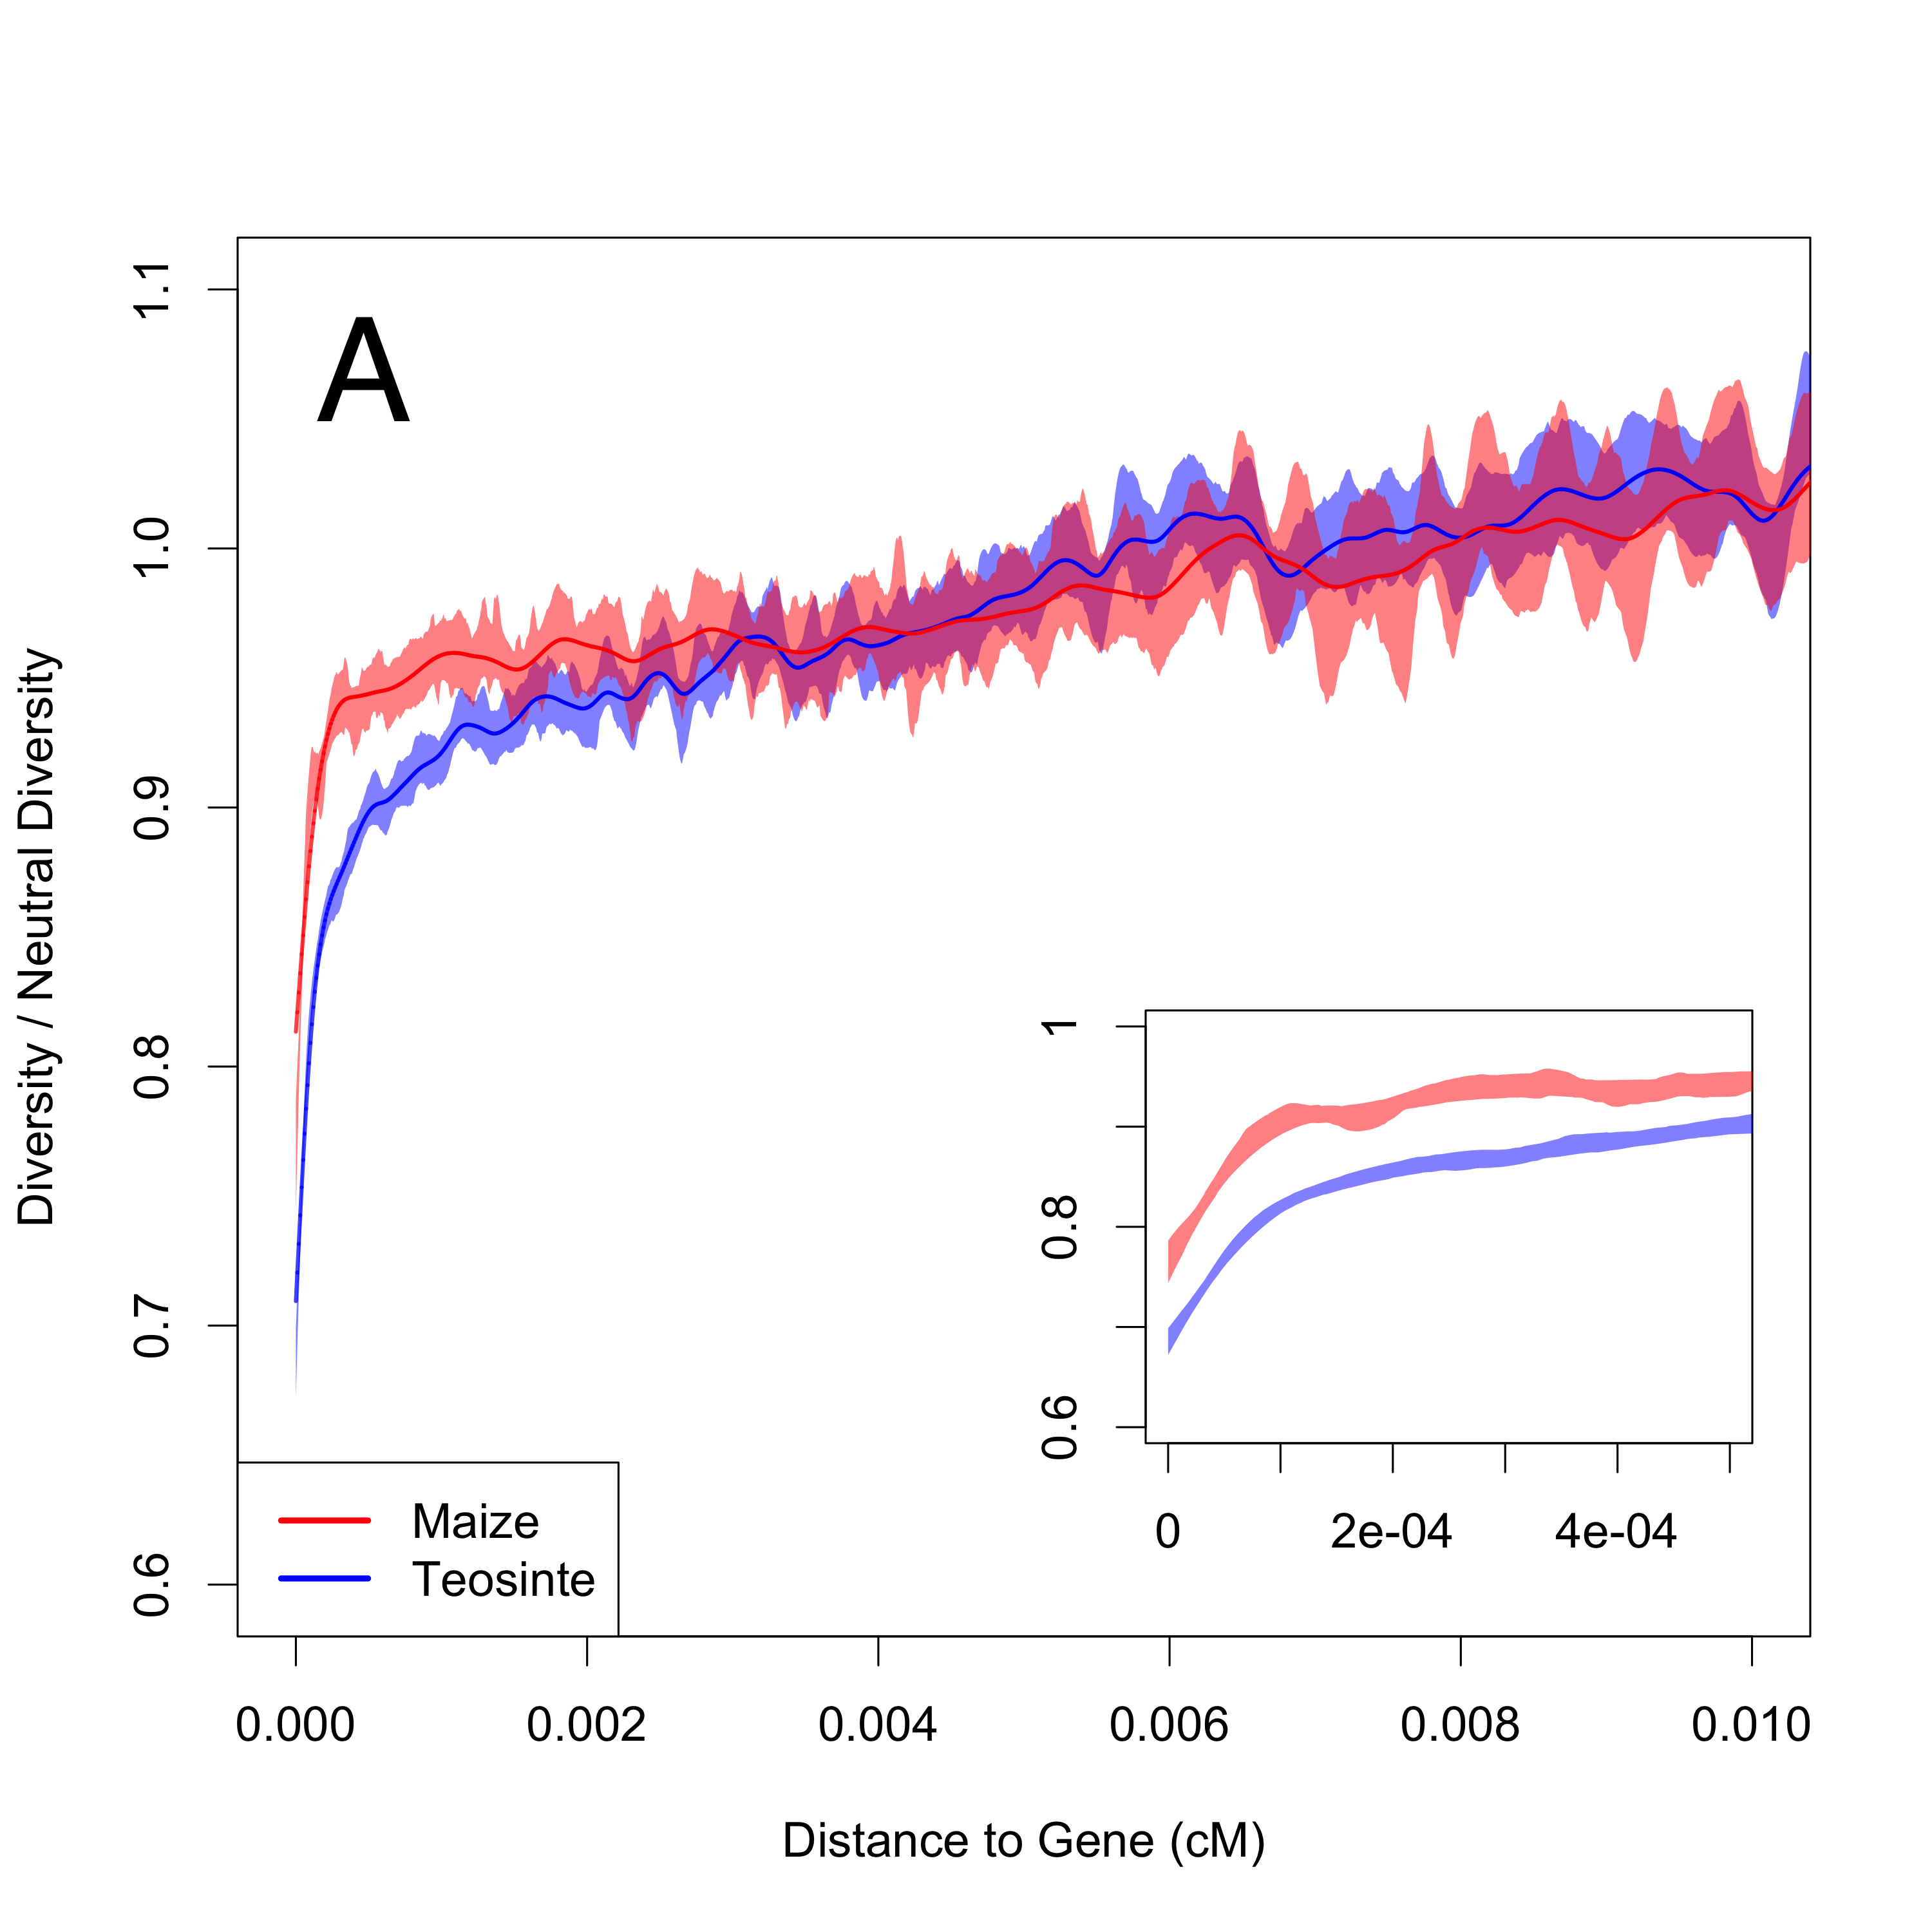
\includegraphics[width=.45\textwidth]{FigsAndFiles/distanceToGene_WithSignificance_Folded2_manuscript.png} 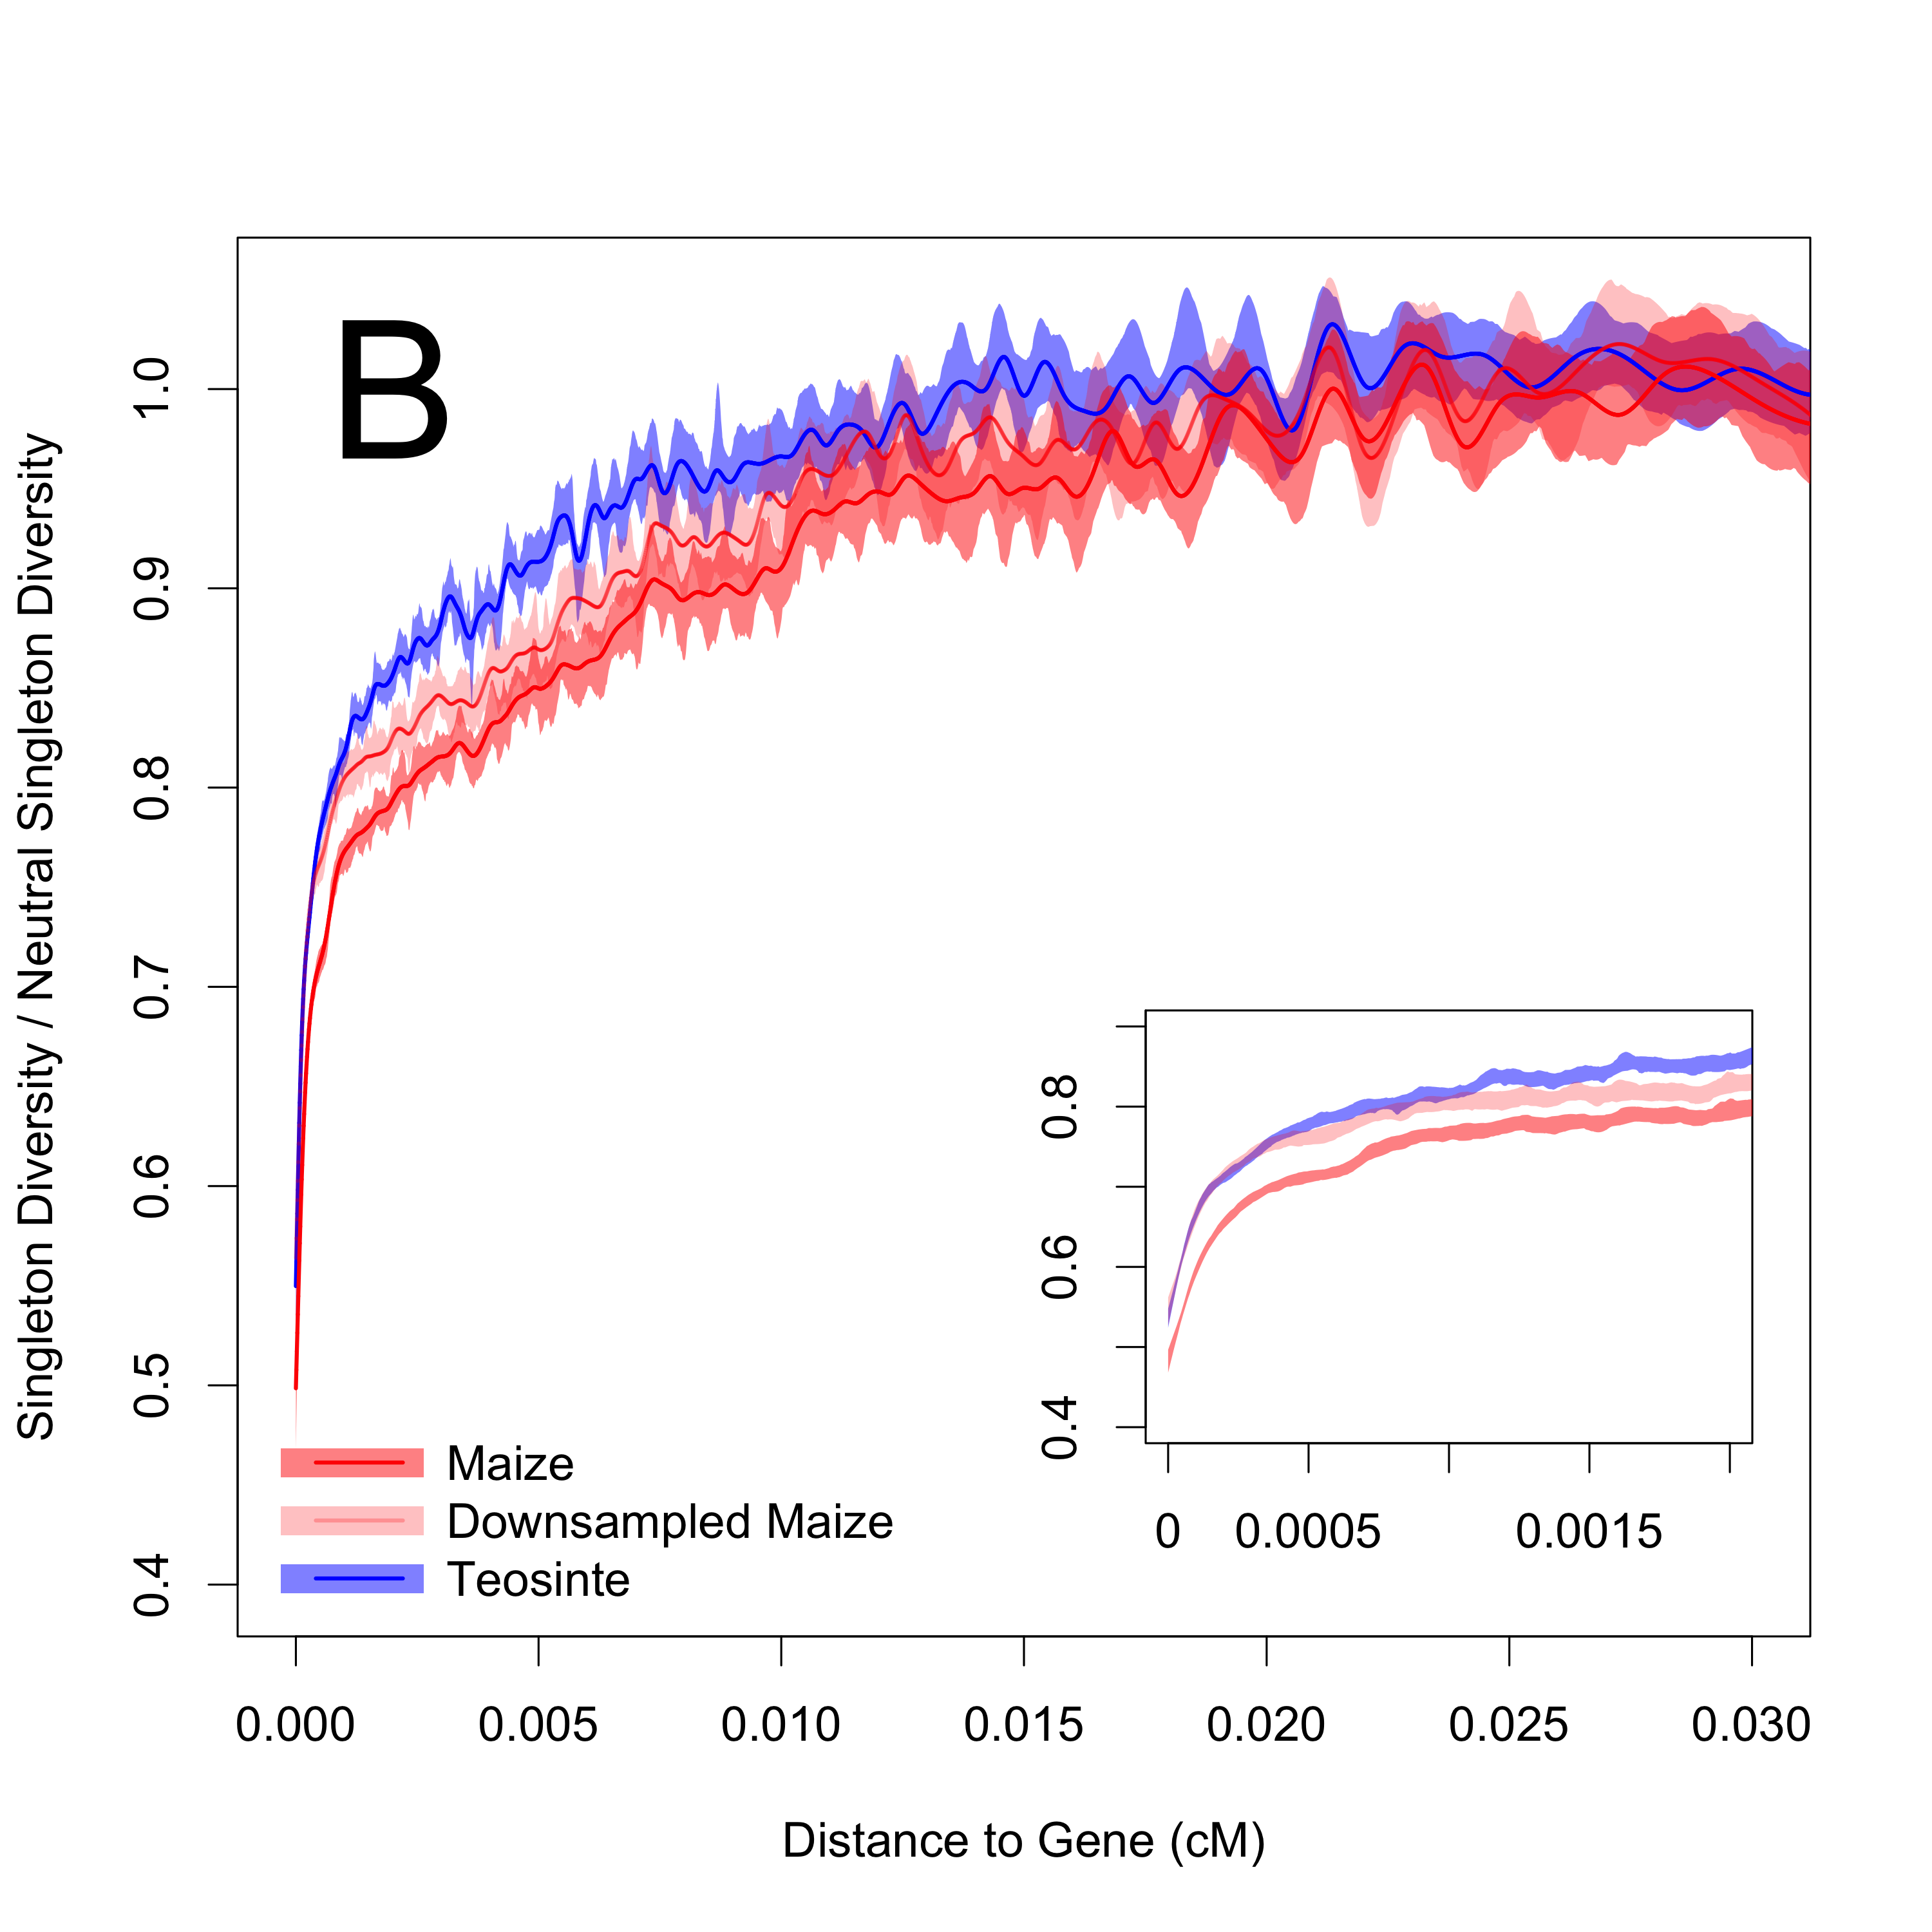
\includegraphics[width=.45\textwidth]{FigsAndFiles/distanceToGene_WithSignificance_Singletons_Downsampled_threeLines_manuscript.png}
\caption{Relative diversity versus distance to nearest gene in maize and teosinte. 
Shown are \textbf{A} pairwise nucleotide diversity and \textbf{B} singleton diversity.  Relative diversity is calculated compared to the mean diversity in windows $\geq 0.01 cM$ or $\geq 0.02 cM$ from the nearest
gene for pairwise diversity and singletons, respectively. 
  Lines depict a loess curve (span of 0.01) and shading represents bootstrap-based 95\% confidence intervals. 
  Inset plots depict a smaller range on the x-axis. \label{fig:purify}
  %\jri{should also add the singleton vs pi comparison within species as a supplemental figure. if $\pi$/singleton curves {\bf don't} match, will need to explain this suggests teosinte not in equilibrium.  good justification i think for msmc model, which we then use to say ``gee whiz, not perfect equilibrium but who cares because the big interesting demography is in maize.''}
  }
\end{figure*}


\subsection{Demography of maize domestication}
To explore whether differences in purifying selection between maize
and teosinte can be explained by demographic processes, we
first estimated the parameters of maize domestication using large-scale
sequencing data involving 23 inbred maize
landraces and 13 teosinte inbred lines included in the HapMap 2 panel
\cite{chia2012}. The maize
lines were collected from across the Americas and the teosinte lines
came from central Mexico. Before estimating demography, we compared
the site frequency spectrum (SFS) in genic and non-genic regions, and
observed substantial differences in the evolution of these classes of
sites. For both maize and teosinte, the SFS within genes showed a
dearth of low-frequency alleles and Tajima's D
\cite{tajima1989} was therefore shifted
to more positive values, as previously shown (Figure \ref{fig:purify}). This is consistent with the aforementioned purifying
selection and indicates that genic regions are not evolving
neutrally. Therefore, for demographic modeling we restricted analysis
to sites at least 5 kb from gene start/stop positions.




We used diffusion approximation as implemented in
$\delta\alpha\delta{i}$ \cite{gutenkunst2009} to find the domestication parameters that best explain
the joint site frequency spectrum of maize and teosinte.  The model we optimized began with an
equilibrium ancestral population of size $N_a$
splitting into separate maize and teosinte populations $T_B$ generations in the past. Moving forward in
time from the split, teosinte maintained the ancestral population size, while
maize experienced an immediate effective population size change to
$N_b$ individuals, followed by exponential growth to size
$N_m$. Additionally, since the split $M_{tm}$ individuals migrated
from teosinte into maize and $M_{mt}$ individuals migrated from maize
to teosinte.

The most likely model suggested an ancestral $\theta$ ($4N\mu$) per base pair of
0.014734, which approximately matches a previous independent estimate \cite{eyre1998}. Assuming a mutation rate of $\mu =
3 \times 10^{-8}$ \cite{clark2005}, this suggests an effective
population size of $N_a = 122,783$ individuals, a population split
$T_B = 15,523$ generations in the past, a maize bottleneck
effective populations size of $N_b = 6,455$ individuals (5.26\% of
$N_a$), a modern maize effective population size of $N_m = 366,973$
individuals, $M_{tm} = 1.35$ migrants per generation from teosinte to
maize, and $M_{mt} = 1.72$ migrants per generation from maize to
teosinte (Figure \ref{fig:bottleneck}). We note that a population
split over 15 thousand generations before present precedes estimates
from
archaeological data, which suggest maize domestication began
no more than 10,000 years before present \cite{smith1995}. This could reflect teosinte population structure that was present before
domestication. Also, note that the genetic time of the population
split must precede physiological changes that could be identified
archaelogically.   Additionally, because recent expansion is
most evidenced by rare alleles, and since our limited sample size provides low
power to detect rare alleles, we expect that the estimate of  $N_m = 366,973$, or $\sim 3N_a$, is likely an underestimate.

Therefore, we utilized a complementary data set of 4,021 maize land-race individuals collected
from across the Americas \textcolor{red}{(SeeDs reference here)} to
obtain a less downward-biased estimate of the current maize effective
population size. According to a singleton-based estimate of $\theta$
\cite{fu1993}, which was utilized since rapid post-bottleneck expansion
implies that rare alleles will most accurately reflect current maize
demography, we obtained the estimate $N_e =
  992,713.5$. Although less biased than the previously mentioned
estimate, we note that ascertainment bias of the
genotyping platform used to generate these data again biases this
estimate downward.

\begin{figure}[!htb]
%\vspace*{.05in}
\centering
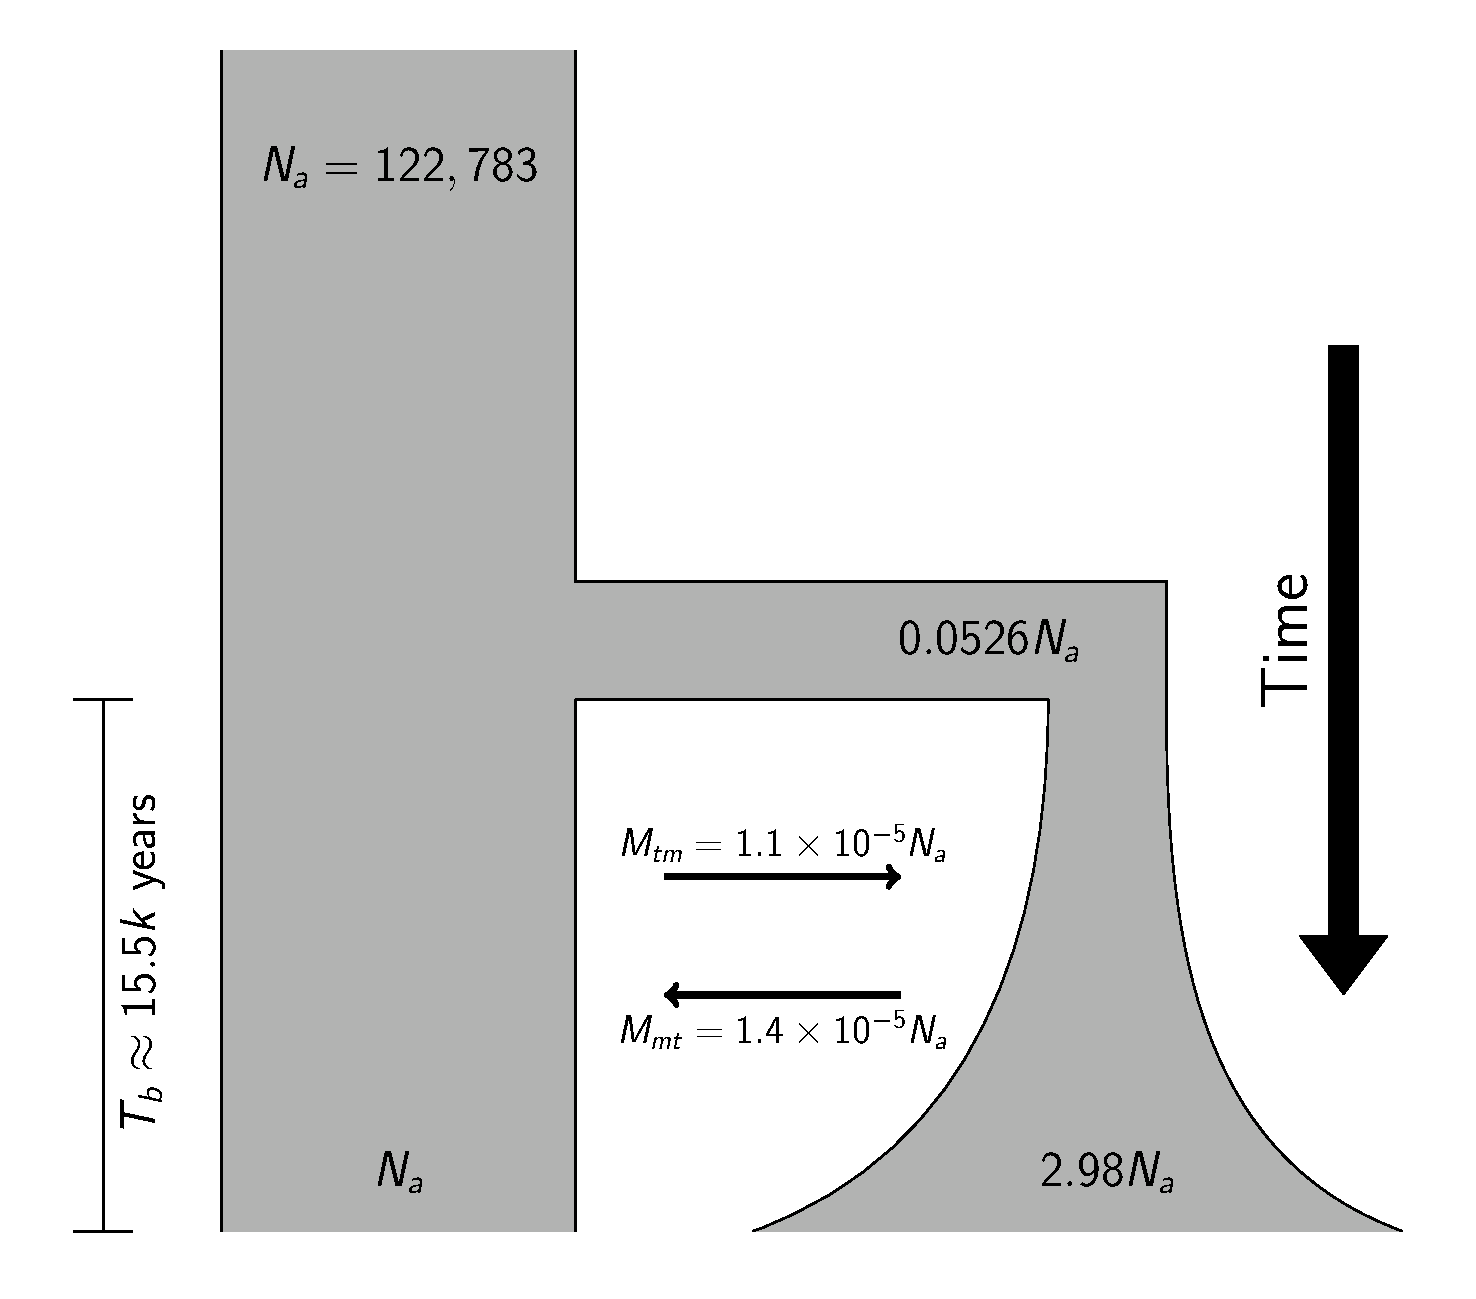
\includegraphics[width=.4\textwidth]{FigsAndFiles/DomesticationModel/domesticationModel.pdf}
\caption{Parameters of domestication as estimated by $\delta\alpha\delta{i}$. Notably,
  the maize effective population size ($N_e$) during the domestication
  bottleneck appears to have consisted of approximately 5.26\%
  the ancestral $N_e$, before recovering two at least 2.98
  times as large as the ancestral $N_e$ \jri{$M_{mt}$ and $tm$ are the reverse of what is described in text}. \label{fig:bottleneck} }
\end{figure}

\subsection{Post-domestication expansion is apparent in patterns of singleton diversity}
Motivated by the rapid post-domestication expansion in maize that is evident from our demographic analysis, we conducted an analysis of genome-wide patterns of singleton diversity. Singleton diversity measures the abundance of alleles that are only observed in one individual among the sample. As a class, singleton alleles depict the most recent patterns of evolution, but
they also have the lowest effect on pairwise diversity. Therefore, unlike
pairwise diversity, patterns of singleton
diversity reflect recent patterns of evolution. Since our sample size
for maize (n=23) was larger than teosinte (n=13), maize singletons were
analyzed directly as well as down-sampled to reflect the sample size of
teosinte. For singletons, our definition of
neutral diversity was defined as diversity at positions at
least 0.02 cM distal from genes. When
evaluating the data in this manner, a very different pattern
emerged compared to what we saw with respect to pairwise diversity. Maize singleton diversity was at least as reduced as teosinte singleton
diversity near genes, but recovered more slowly
(Figure \ref{fig:purify}), implying that in the
recent past maize has been more influenced by purifying selection than has
teosinte.

Together, these findings suggest that demographic history has
a strong influence on the effect of purifying selection. Historically,
teosinte has had a larger population size than maize, and only
recently has maize population size overcome that of teosinte. Since
the efficacy of purifying selection scales with population size,
these results likely reflect changes in $N_e$ more than they reflect
underlying changes in selection pressure.

Similarly, to complement our investigation of pairwise diversity surrounding substitutions, we studied patterns of singleton diversity surrounding synonymous and non-synonymous substitutions in maize (Figure \ref{sFig:singleton}). A nearly identical pattern to that shown in Figure \ref{fig:hardSweeps} was observed. This further demonstrates that even the most recent selection patterns in maize are not dominated by hard sweeps.



\subsection{Purifying selection results are robust to soft-sweeps}
As a category, instances of soft-sweeps, or cases of selection on alleles that have already reached intermediate frequency before becoming advantageous, are difficult to identify \cite{wilson2014}. However, this form of selection is likely to be frequent during crop domestication \cite{innan2004}. We were concerned that the disparate patterns of pairwise and singleton diversity in maize and teosinte, which seem to reflect differences in the efficiency of purifying selection due to demographic history, may instead reflect differences in the location and abundance of soft-sweeps. Therefore, we re-analyzed patterns of pairwise and singleton diversity in maize and teosinte including only a subset of sites that are least likely to correspond to soft-sweeps. To achieve this, we performed a genome-wide scan for soft or hard sweeps in maize or teosinte based on the H12 statistic \cite{garud2015}. H12 is sensitive to both hard and soft sweeps. Sites nearest to genes that displayed among the top 20\% of H12 values in either maize or teosinte were removed from our data set, and both pairwise and singleton diversity at remaining sites, as a function of the distance to the nearest gene, was calculated (Figure \ref{sFig:H12}). This subset of the data is no longer subject to the potentially confounding effects of soft-sweeps, and nearly identical patterns of pairwise and singleton diversity surrounding genes are observed. This provides further evidence that the patterns of diversity we observe in maize as compared to teosinte are the result of rapid population expansion as opposed to differing selective patterns in the domesticated and wild taxa.

\section{Discussion}
\subsection{Little positive selection on new genic mutations}
\jri{mention divergence time from \emph{Tripsacum}, roughly 1-1.2 million years before present \cite{ross2009}.}Our findings indicate that hard selective sweeps have not contributed substantially to genome-wide patterns of diversity in maize. More specifically, we observe that positive selection on new genic mutations in maize is not common compared to other drivers of diversity. This finding does not exclude the possibility that hard sweeps have taken place at non-genic sites, such as in those in enhancer regions. One known example of positive selection on a non-genic mutation involves the \emph{tb1} locus of maize, which is one of the best characterized examples of positive selection on a ``domestication gene'' in any crop \cite{clark2006}. However, the maize \emph{tb1} allele was already present in teosinte before domestication \cite{studer2011}, so this this example is in agreement with our finding that hard sweeps are rare. The \emph{gt1} locus is another well-characterized case of positive selection operating on standing variation at an enhancer region \cite{wills2013}. Instances of selection on standing variation such as these, often called soft sweeps, may be a major contributor to maize patterns of diversity \cite{beissinger2014}, and this could be part of the explanation as to why hard sweeps appear to be so rare, despite obvious morphological differences between maize and teosinte.

Unfortunately, our ability to accurately identify soft sweeps, and particularly to distinguish them from hard sweeps, remains limited \cite{innan2004,messer2013}. However, we implemented a scan based on the H12 statistic, which is designed to identify both hard and soft sweeps with reasonable power \cite{garud2015}. Although the goal of this study was not to identify specific sweeps, it may be that the outlier sites distinguished by H12 are primarily composed of soft sweeps instead of hard. Similarly, previous studies scanning for evidence of positive selection in maize \cite{hufford2012} may have picked up primarily evidence of soft sweeps. In domesticated species, artificial selection beginning at the onset of domestication represents a drastic shift in selective pressure. One can easily imagine a scenario in which previously neutral or slightly deleterious variants that were segregating in the population when this shift took place suddenly became beneficial, leading to soft sweeps. As appealing as this explanation is, however, our data do not speak to the abundance of soft sweeps, beyond demonstrating that they are one possibility for the lack of observed hard sweeps.

We should additionally note that our observations do not exclude the possibility of infrequent hard sweeps having taken place during maize evolution. In fact, the maize locus \emph{tga1} that has been shown to correspond to a hard sweep at an amino-acid changing mutation \cite{wang2015}. Surrounding \emph{tga1},  our data demonstrate a pattern consistent with a hard sweep. But, our data demonstrate that instances such as this are infrequent. This contrasts sharply with \emph{Drosophila} \cite{sattath2011} and \emph{Capsella} \cite{williamson2014}, where differences in diversity surrounding synonymous and non-synonymous substitutions are clear suggesting hard-sweeps are abundant. However, it agrees with what has been seen for humans \cite{hernandez2011}. 

\subsection{Demography of domestication}
\jri{add note that demography inference will require regions far from genes, compare to \cite{wright2005,wang1999,eyre1998}. cite some theory or empirical paper showing this to be the case in humans/drosophila}
Since we observed that classical hard sweeps do not explain patterns of maize diversity, it is perhaps unsurprising that we instead found evidence of demographic history contributing substantially to genetic diversity. Our estimate of the demographic history of maize, which is the first estimate of maize demographic history to utilize whole-genome-sequence (WGS) data, allowed us to disentangle the confounding parameters of bottleneck strength and bottleneck intensity. This confounding limited previous domestication estimates \cite{wright2005}. By utilizing the two-dimensional site frequency spectrum (SFS) between maize and teosinte for inference \cite{gutenkunst2009} we estimate that the maize effective population size during the bottleneck was approximately 5\% that of teosinte. A bottleneck of this magnitude may have enabled moderately deleterious alleles to reach intermediate frequency in maize, while also increasing the probability that strongly deleterious alleles segregating at low frequency in teosinte were purged from the maize gene pool, due to elevated drift as is predicted during a domestication bottleneck \cite{tajima1989}.

After the initial bottleneck, our analysis suggests that maize $N_e$ expanded to reach levels much greater than that of teosinte. Our WGS-based estimate shows that the $N_e$ of landrace maize is at least 3X that of ancestral teosinte, while our singleton-based estimate from the the SeeDs project data \textcolor{red}{(citation)} implies an $N_e$ of close to 1 million individuals, or $\sim$8X that of ancestral teosinte. From the perspective of a new mutation, both of these estimates are biased downward, since they represent past reductions in diversity due to the aforementioned bottleneck. A back-of-the-envelope calculation of modern $N_e$ can be made by assuming there are 47.9 million ha of landrace maize in production \cite{cimmyt1999}, 42,000 plants per ha for open pollinated maize varieties \cite{van2010}, and conservatively that no more than one in 1,000 plants contribute gametes to the next generation. This calculation implies a modern $N_e \geq  2$ billion individuals, and incorporates no individuals from hybrid breeding programs. If for some reason this back-of-the-envelope calculation is an overestimate, even by several orders of magnitude, it is clear that the post-domestication expansion in maize $N_e$ is enormous. Patterns of singleton diversity in maize, as discussed in more detail in the next section, demonstrate that this recent expansion has a notable impact on the maize genome.


\subsection{Demography strongly impacts efficiency of purifying selection}
The observation that maize pairwise diversity is less impacted by the distance to the nearest gene than is teosinte pairwise diversity is reasonable from a long-term evolutionary standpoint. Theory has established that purifying selection is more efficient in a large population than in a small one \cite{kimura1984}, and this observation most likely reflects that prediction. More specifically, if teosinte $N_e$ remained relatively constant while maize bottlenecked and recovered exponentially, this provides that the average $N_e$ of maize over the previous several thousand generations is much smaller than that of teosinte, regardless of how much maize has ballooned in the recent past. Therefore, our observation shows that purifying selection in maize has not purged deleterious alleles, or the neutral alleles they are linked to, as effectively as in teosinte.

The reversal of this trend when we analyze only singleton diversity instead of pairwise diversity, however, stands out as a notable observation. Every mutation begins as a singleton (an allele present in only one individual), and therefore singletons are, on average, the youngest class of alleles that can be observed. Therefore unlike pairwise patterns of diversity, which are most heavily influenced by intermediate frequency alleles based on the definition of $\pi$ \cite{nei1979}, singleton diversity is most influenced by recent patterns of evolution. Hence, because our demographic estimation indicates dramatic expansion of maize $N_e$ in the recent past, we expect for purifying selection to presently operate more efficiently in maize than in teosinte. This observation is very clearly demonstrated by the fact that singleton diversity in maize is more impacted by the distance to the nearest gene than it is in teosinte, as was shown in Figure \ref{fig:purify}.

A consequence of the inefficient purifying selection that maize experienced during its bottleneck is likely that it harbors more deleterious alleles segregating at intermediate frequency than does teosinte. This could be a part of the explanation of why maize inbreds have continued to improve over the past several decades \cite{meghji1984}; if deleterious alleles tend to be recessive and are particularly frequent, they will have ample opportunities to display their phenotypes in inbreds. Our results also demonstrate that recent purifying selection in maize has become much more effective, potentially explaining the ongoing improvement of these inbreds as maize lines are continuously select

Ultimately, we have shown that purifying selection in maize has operated very differently than purifying selection in teosinte. This observation, along with the potential for soft sweeps, appear to explain the phenotypic divergence \jri{pretty hard to argue that purifying selection explains phenotypic divergence!} between maize and teosinte much more completely than does positive selection generating hard-sweeps at protein-coding mutations. Importantly, our estimation of the parameters of the maize domestication bottleneck contribute to the understanding of how the demography of crop domestication can impact crop diversity. The bottleneck-effects from a sudden collapse in population size have been well studied and are known to impact crops for thousands of generations. Complementing this knowledge, our results demonstrate that the rapid expansion experienced by many crops after domestication can also have a profound influence on patterns of diversity, and the effects of this expansion should be accounted for as important contributors to long-term evolution.

\begin{materials}

  \subsection{BASH, R, and Python scripts}
All scripts used for analysis are available in an online repository at \textcolor{red}{REPO ADDRESS HERE.} 

\subsection{Plant materials}
We made use of published sequence of inbred accessions of teosinte (Z. \emph{mays} ssp. \emph{parviglumis}) and maize landraces from the Maize HapMap2 panel \cite{chia2012, lemmon2014}. 
We removed \X teosinte and \X maize individuals that appeared as outliers in an initial principal component analysis  (Figure \ref{sFig:PCA}), leaving 13 teosinte and 23 maize that were used for all subsequent analyses (Table \ref{sTab:list}).

\subsection{Physical and genetic maps}
Sequences were mapped to the maize B73 version 3 reference genome \cite{schnable2009} (ftp://ftp.ensemblgenomes.org/pub/plants/release-22/fasta/zea\_mays/dna/) as described by \cite{chia2012}.\jri{did we use their bams? I thought we used bwa bams, which are not listed and weren't used for hapmap2. if that's the case, we need to mention this difference and acknowledge Robert for providing those bams. either way, we need to include a link to the bamfiles too. somewhere here or above mention URL for Tripsacum bams. did we align those too or download someone else's?}
All analyses made use of uniquely mapping reads with mapping quality score $\geq  30$ and bases with base quality score $\geq 20$; quality scores around indels were adjusted following \cite{li2011statistical}.
We converted physical coordinates to genetic coordinates via linear interpolation of the 1cM resolution NAM genetic map \cite{glaubitz2014}, \jri{i thought this should be wallace not glaubitz? need to specify what you do with physical positions before and after last marker on each chrom and markers, if any, that have physical and genetic order that disagree}.

\subsection{Estimating the site frequency spectrum}
We estimated both the genome-wide site frequency spectrum (SFS) as well as a separate SFS for genic (within annotated transcript) and intergenic ($\geq 5kb$ from a transcript) regions. 
We used the biomaRt package \cite{durinck2009,durinck2005} of R \cite{R2014} to parse annotations from the \X annotation \jri{include annotation version number and link to ENSEMBL annotation used}. 
We estimated single population and joint SFS with the software ANGSD \cite{korneliussen2014}, including all positions with at least one aligned read in $\geq 80\%$ of samples in one or both populations.
We assumed individuals were fully inbred and treated each line as a single haplotype. \jri{i removed options details because they don't make sense to casual reader and the interested reader can find the script. }
Because ANGSD cannot calculate a folded joint SFS, we first polarized SNPs using the maize reference genome and then folded spectra using $\delta\alpha\delta{i}$ \cite{gutenkunst2009}.

\subsection{Demographic inference}
We used the software $\delta\alpha\delta{i}$ \cite{gutenkunst2009} to estimate parameters of a domestication bottleneck from the joint maize-teosinte SFS.
We modeled a teosinte population of constant effective size $N_a$, that at time $T_b$ generations in the past gives rise to a maize population of size $N_b$ which grows exponentially to size $N_m$ in the present (Figure \ref{fig:bottleneck})
The model includes migration of $M_{mt}$ individuals each generation from maize to teosinte and $M_{tm}$ individuals from teosinte to maize.  
We fixed $N_a$ using $\delta\alpha\delta{i}$'s estimation of $\theta=4N_a\mu$ from the data and a mutation rate of $3 \times 10^{-8}$ \cite{clark2005}. 
We estimated all other parameters using 1,000 $\delta\alpha\delta{i}$ optimizations and allowing initial values to be randomly perturbed by a factor of 2.  
Initial values and upper and lower bounds can be found in table \X. \jri{this looked terrible in text, please make a supp. table.  keep track of notation as e.g. we explain $N_b$ as population size of bneck, but in reality parameter we fit is $\frac{N_b}{N_a}$}
%, setting initial parameter values at $\frac{N_b}{N_a}=0.02$, $\frac{N_m}{N_a}=3$, $\frac{T_b}{2N_a}=0.04$, and $\frac{M_{mt}}{N_c}=\frac{M_{tm}}{N_a}=10^{-5}$, where the maize population size $Nc$ at time $i$ generations in the past is $N_c=N_ae^{\frac{ln(\frac{N_m}{N_a})(T_b-i)}{T_b}}$.
%\jri{make sure these are right (e.g. is it 2Na or 4Na for Tb?). note that we have to redo this in fractions or words because above you call Nb a population size when in reality we are estimating a proportion}
%We allowed initial values to be , and set upper and lower bounds such that $10^{-7} \leq \frac{N_b}{N_a} \leq 2$, $10^{-7} \leq \frac{N_m}{N_a} \leq{200}$, $0 \leq \frac{T_b}{2N_a} \leq 1$, $10^{-10}\leq \frac{M_{tm}}{N_a}\leq 10^{-3}$, and $10^{-10}\leq \frac{M_{mt}}{N_c}\leq 10^{-3}$
We report parameter estimates from the optimization run with the highest log-likelihood.

We further made use of a large genotyping data set of more than 4,000 maize landraces \cite{Hearne2015} to estimate the modern maize $N_e$ from singleton counts.
We filtered these data to include only SNPs with data in $\geq 1,500$ individuals, and then projected the SFS down to a sample of 500 individuals.\jri{cite or mention how projection was done}. 
We then estimated $N_e$ from the data assuming $\mu = 3 \times 10^{-8}$ \cite{clark2005} and the relation  $4N_e\mu = \frac{S}{L}$ \cite{fu1993}, where where $S$ is the total number of singleton SNPs and $L$ is the total number of SNPs in the dataset.

Finally, \jri{MSMC text here}

\subsection{Diversity}
We made use of the software ANGSD \cite{korneliussen2014} for diversity calculations and genotype calling. 
We calculated diversity statistics in maize and teosinte in 100bp non-overlapping windows using filters as described above for the SFS. \jri{this said 1,000 kb which is 1Mb, but should say 100bp right?}
We used allele counts to estimate the number of singleton polymorphisms in each window, and used binomial sampling to create a second maize data set down-sampled to have the same number of samples as teosinte.
We called genotypes in maize, teosinte, and \emph{Tripsacum} at sites with a SNP p-value $<10^{-6}$ and when the genotype posterior probability $>0.95$.
We identified substitutions in maize and teosinte as all sites with a fixed difference with \emph{Tripsacum} and $\leq 20\%$ missing data. 
Substitutions were classified as synonymous, missense, or noncoding using the ensembl variant effects predictor \cite{mclaren2010}.
For each window with $\geq 100bp$ of data we computed the genetic distance between the window center and the nearest synonymous and missense substitution as well as the genetic distance to the nearest gene transcript. \jri{this said gene center, but we're not using gene center anymore, right?} 

%Teosinte diversity is
%generally higher then maize diversity. Therefore, to enable comparisons between
%the reduction of diversity around genes in maize and teosinte, a
%neutral measure of pairwise and singleton diversity for each taxa was
%estimated. For pairwise diversity, this neutral measure was defined according to
%mean pairwise diversity at windows greater than 0.01 cM from the nearest
%gene. For singletons, both maize and teosinte still showed reduced
%diversity at a distance of 1 cM, so neutral diversity in this case was
%defined as mean singleton diversity at positions 0.02 cM or greater
%from genes. Then, pairwise and singleton diversity at each window was
%standardized by dividing by the corresponding neutral
%measure. Separately for pairwise and singleton diversity in maize and
%teosinte, . Significant differences were assessed by taking 100 bootstrap
%samples from each set of diversity windows and re-fitting the cubic smoothing spline to each. Then, the
%2.5\% and 97.5\% quantiles of values along the bootstrapped splines
%were identified.

%To verify that this approach is robust to reduced power at highly conserved sites \cite{enard2014}, we applied the method to subsets of sites that included only positions nearest to the  most- or least-conserved 10\% of genes data. This was achieved by assigning every gene a GERP score corresponding to the average score observed across it \cite{rodgers2015}. Next, genes in the top and bottom 10\% quantiles of GERP score were isolated. Two datasets were created, each including all diversity windows who's nearest gene was in the high or low GERP score sets. Finally, Loess fits of diversity vs. distance to gene were computed from sites within each GERP score.

%In addition  next Two types of diversity surrounding genes were investigated. The first
%was pairwise diversity in 1kb windows, as described previously. The
%second was singleton diversity in 1kb windows. Singletons represent
%the rarest class of alleles that this dataset can identify, and
%collectively demonstrate the most recent patterns of evolution. Minor
%allele frequencies were estimated with ANGSD \cite{korneliussen2014} using the
%same quality filters previously described. Then, the number of
%singletons in each non-overlapping 1kb window was calculated with R
%for both maize and teosinte \cite{R2014}. For maize, we also generated a parallel set of downsampled
%singleton data, for which binomial sampling within R was conducted
%based on allele frequencies at each site, to generate a singleton
%psuedo dataset of sample size 13, equivalent to our sample size for
%teosinte. BiomaRt \cite{durinck2009, durinck2005} was then used to identify
%the center of each gene. Next, the distance from each diversity window center
%to the nearest gene center was computed.

\subsection{Selection scan}
We scanned the genome to identify sites that have experienced recent positive selection using the H12 statistic \cite{garud2015} in sliding windows of 200 SNPs with a step of 25 SNPs.


%JRI IDEAS:
% look at SFS of SNPs by GERP score in maize vs teosinte. shift to lower freq. should be seen at lower GERP scores in maize
% discuss our estimates of deleterious mutation rate from B stuff.  these suggest only ~25% of mutations are deleterious, which contrasts results from a standard DFE
% do a standard DFE! this gives us the proportion of mutations in categories of Ns. Can use Eyre-Walker software.
% i think we do need to say something about load. add up GERP scores like Li?


\end{materials}

\begin{acknowledgments}
We are indebted to Graham Coop and Simon Aeshbacher for their constructive input during this study. Funding was provided by NSF Plant Genome Research Project 1238014.
\end{acknowledgments}

\bibliography{Reference}
\bibliographystyle{pnas}

\onecolumn
\section*{Supporting Information}
\renewcommand\thefigure{S\arabic{figure}}    
\setcounter{figure}{0}


\begin{figure}
  \begin{center}
    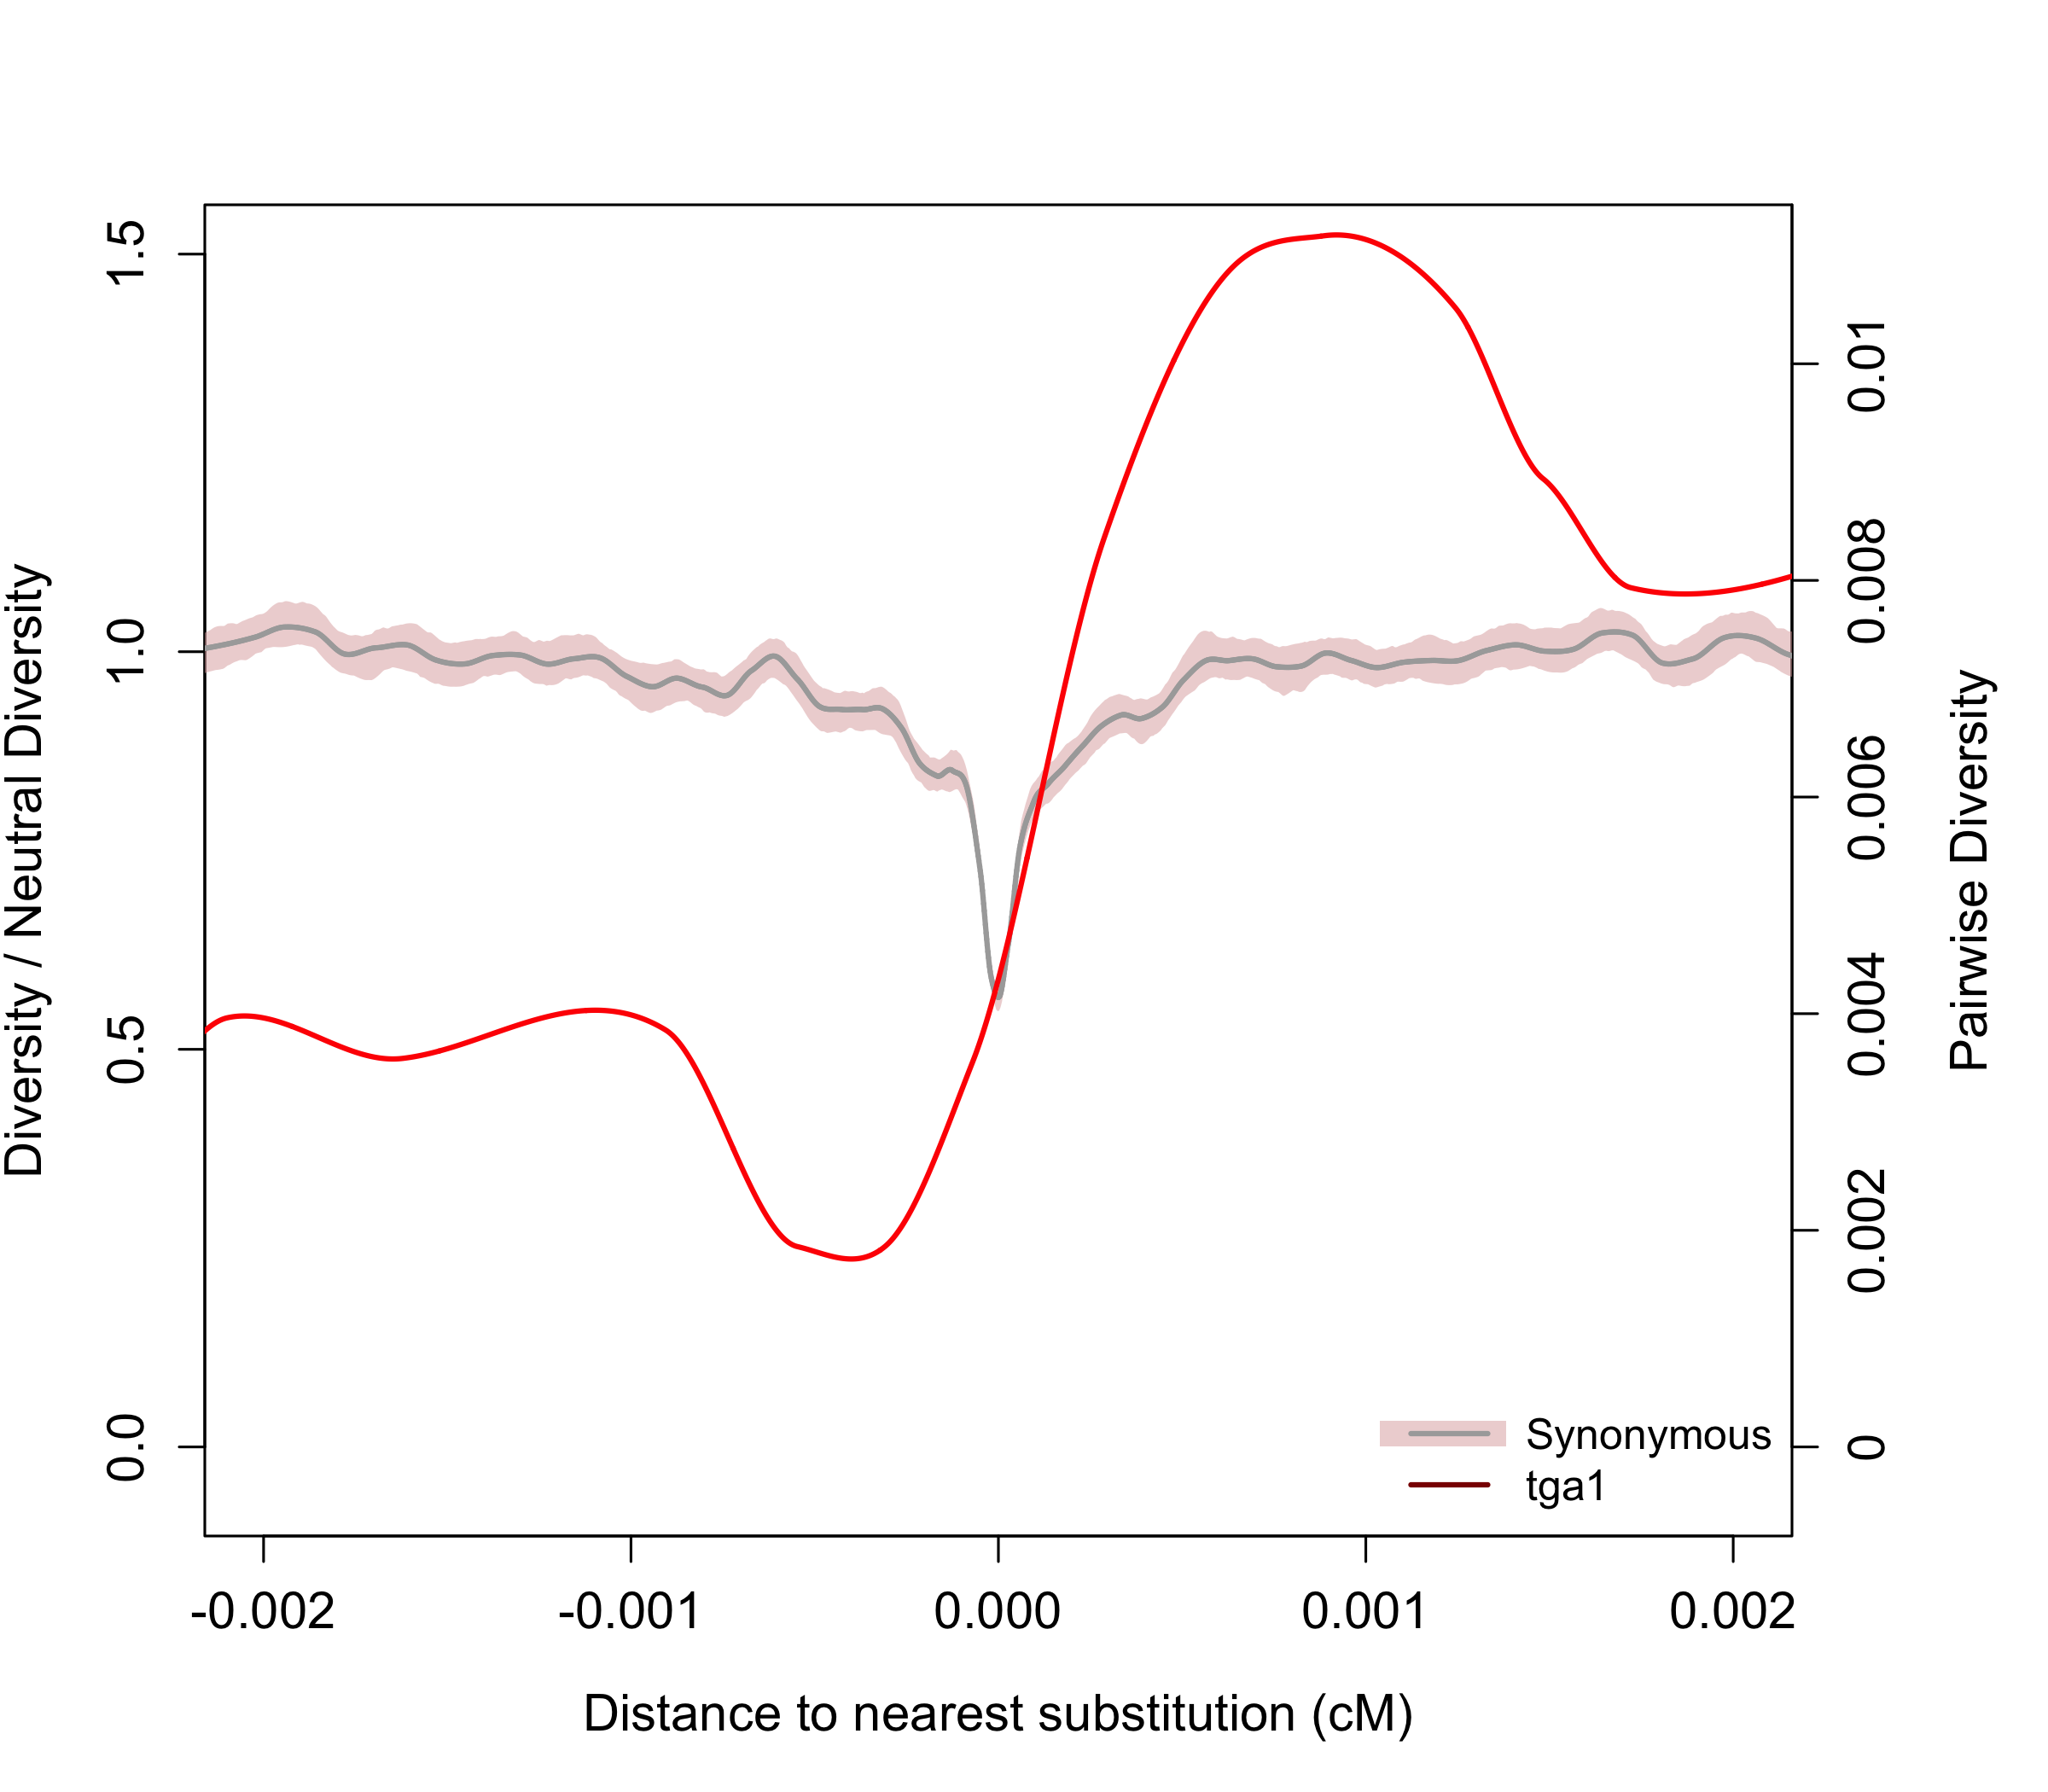
\includegraphics[width=.85\textwidth]{FigsAndFiles/plotDiversity_TvM_Folded2_Significance_tga1Supp_June.png} \\
    \end{center}
\caption{Diversity surrounding the causitive polymorphism at the \emph{tga1} locus is plotted. Since this is only one gene, the large amount of noise compared to our average plots is expected. However, notice that diversity precisely at the causitive polymorphism is reduced and a recovery of diversity is observed away from that site. \label{sFig:tga1}}
\end{figure}
\clearpage


\begin{figure}
  \begin{center}
    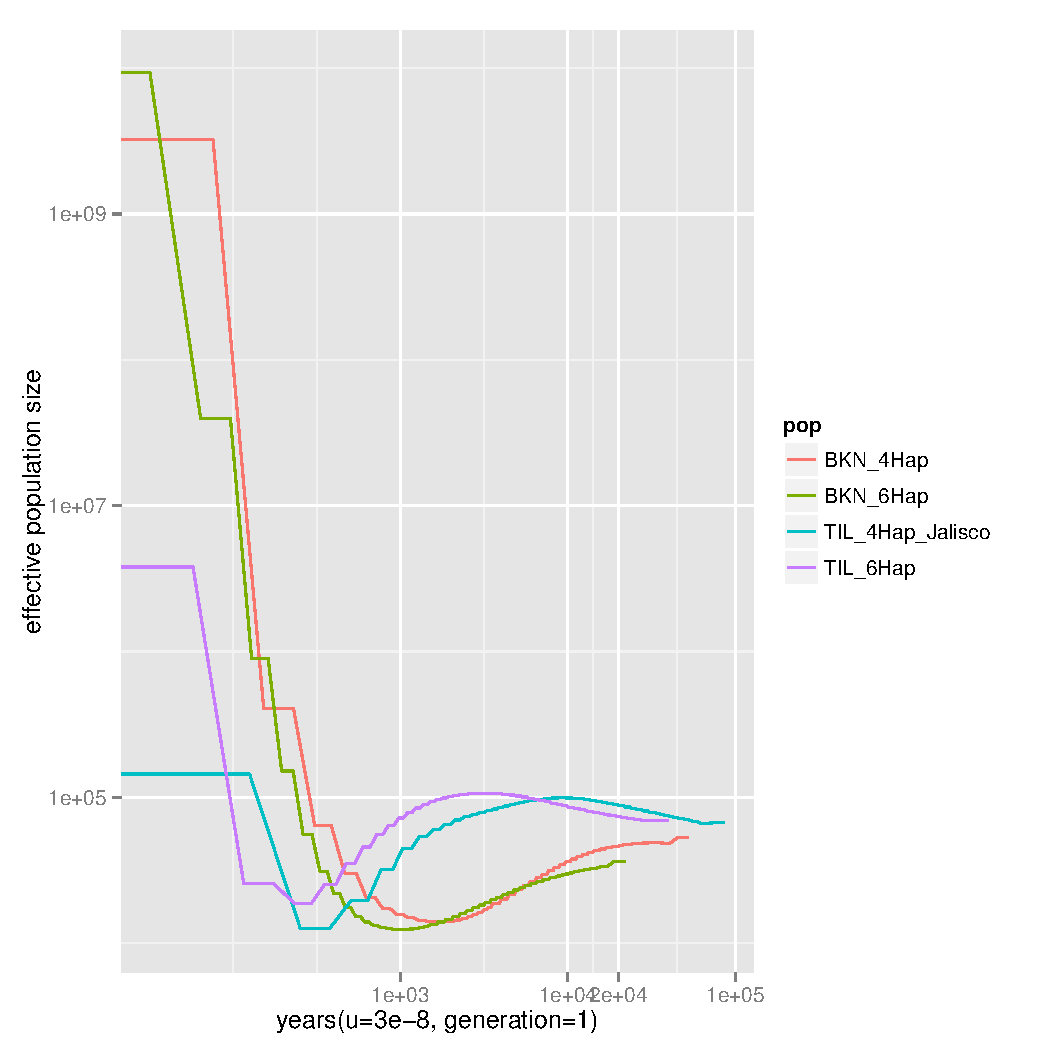
\includegraphics[width=.85\textwidth]{FigsAndFiles/BKN.TIL.msmc.pdf} \\
    \end{center}
\caption{\jri{need MSMC caption} \label{sFig:msmc}}
\end{figure}
\clearpage


\begin{figure}
  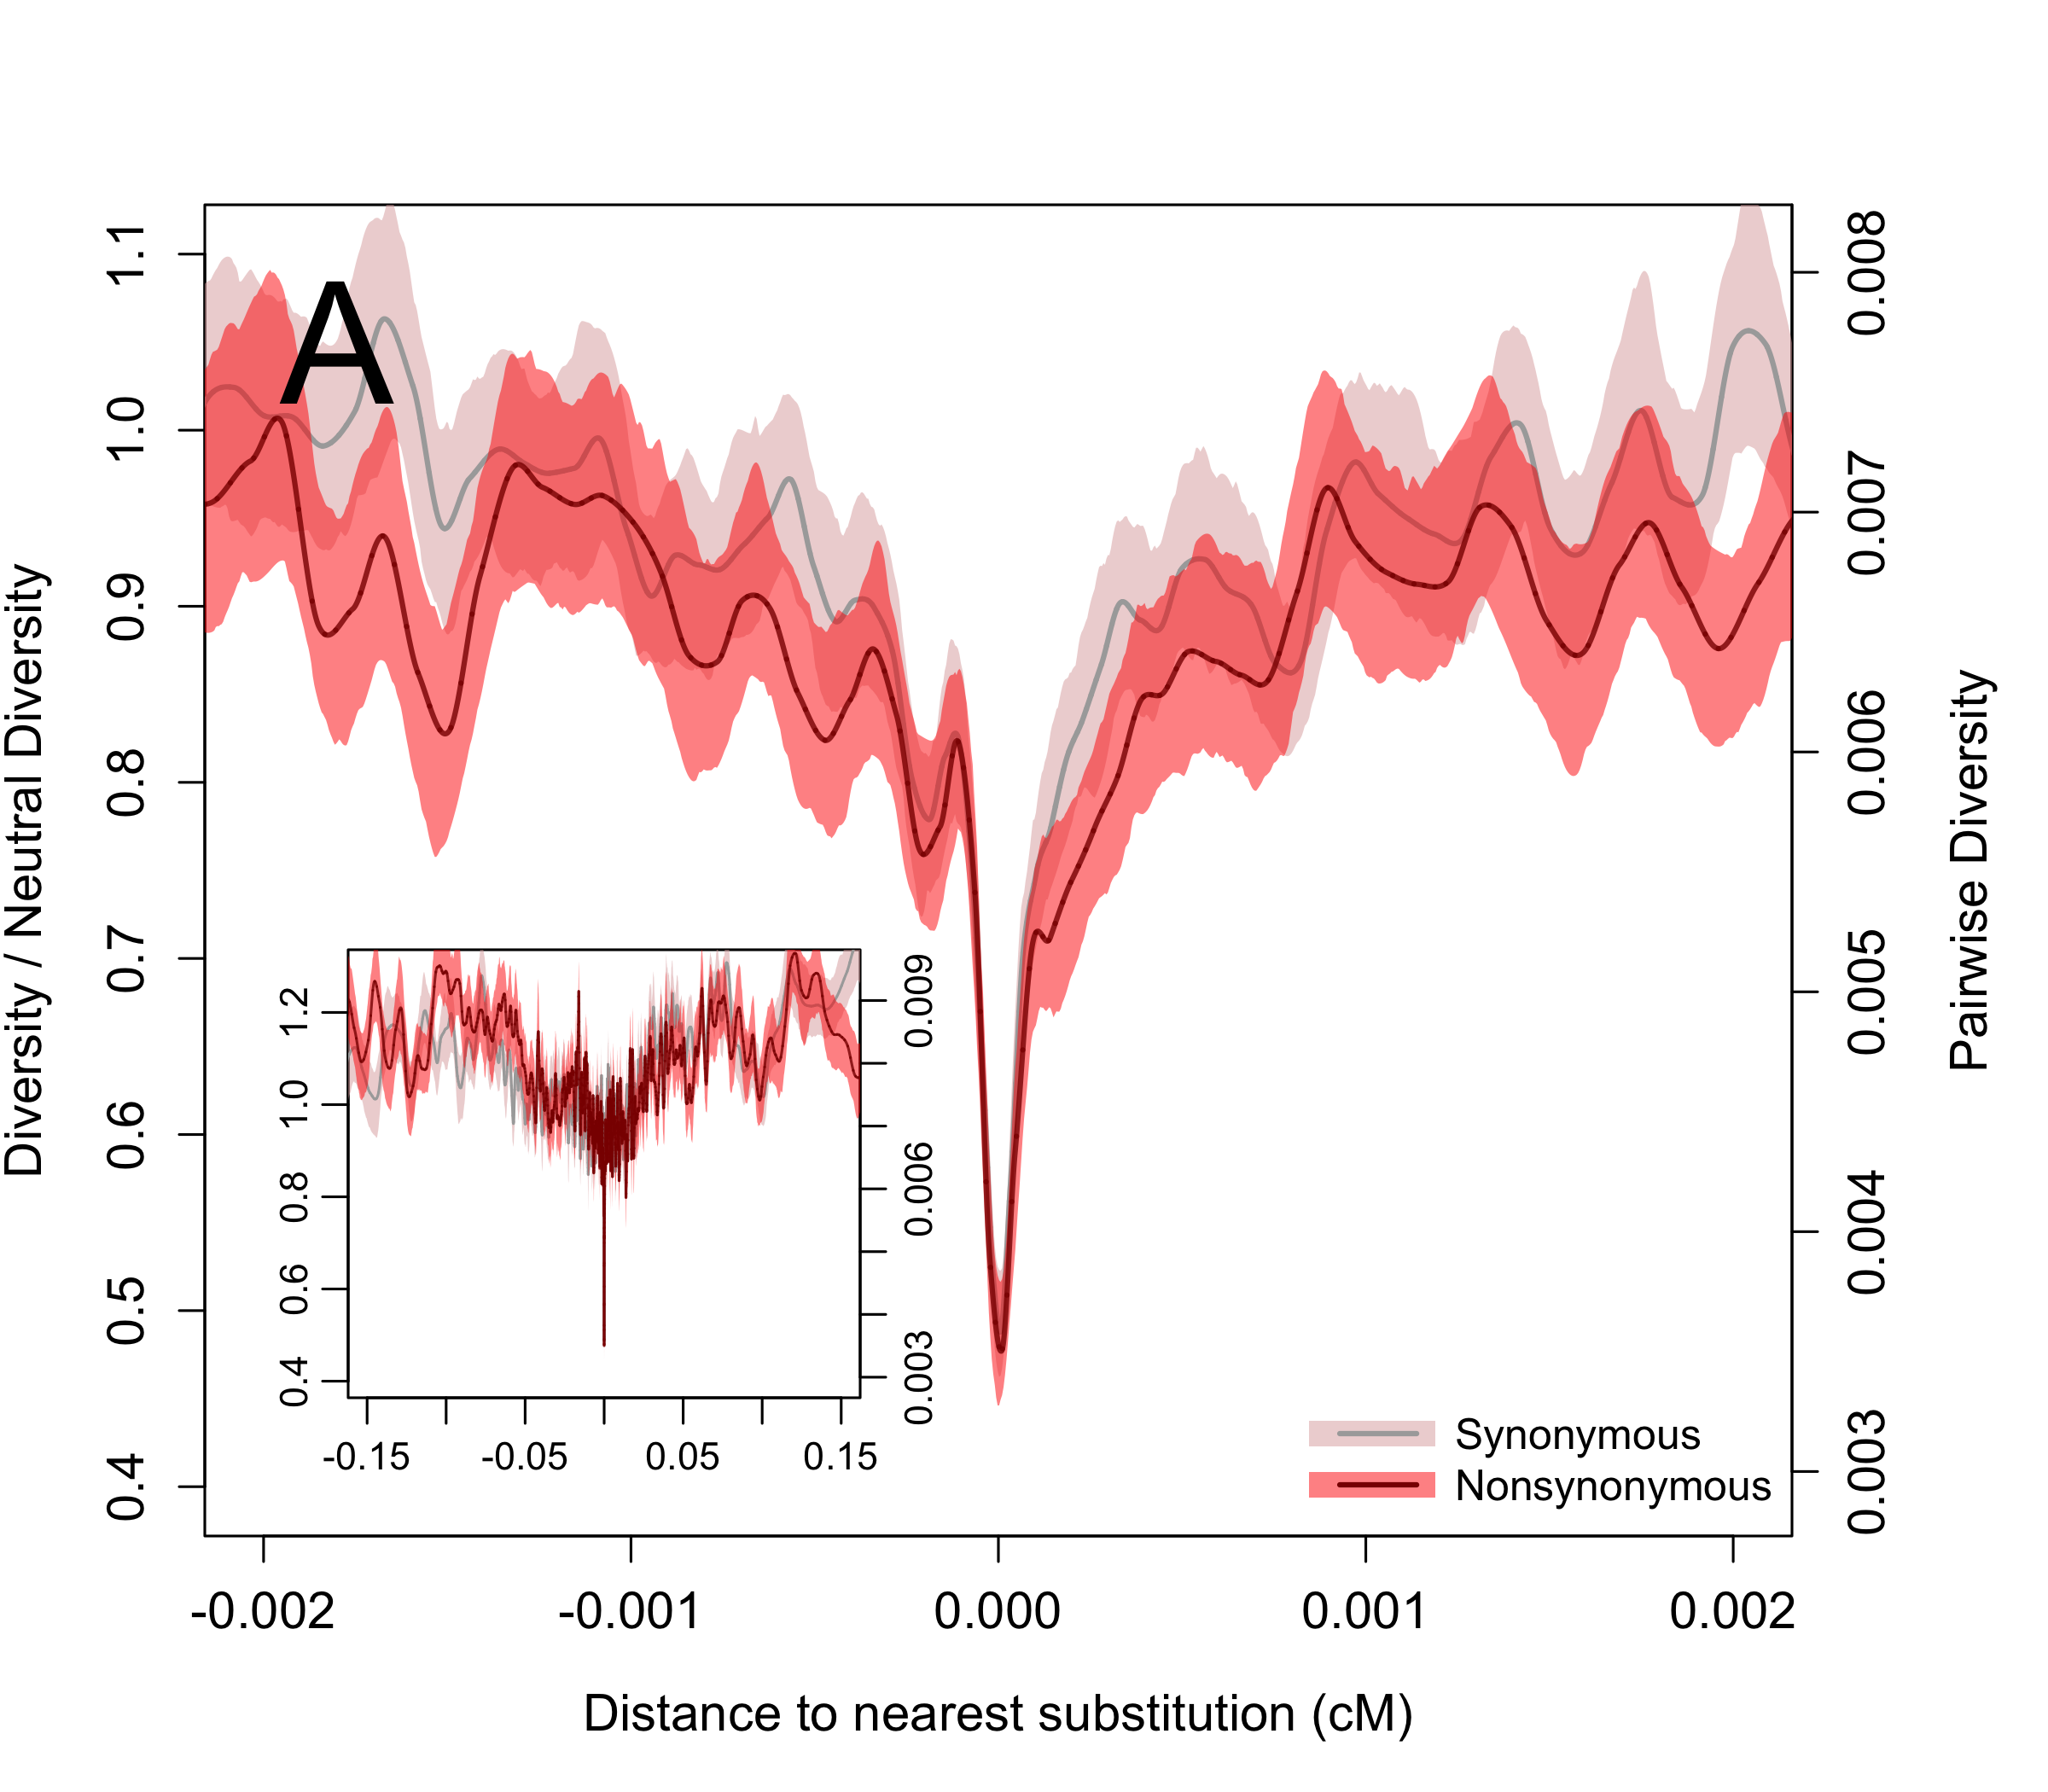
\includegraphics[width=.5\textwidth]{FigsAndFiles/plotDiversity_TvM_Conserved_Significance_June.png}
  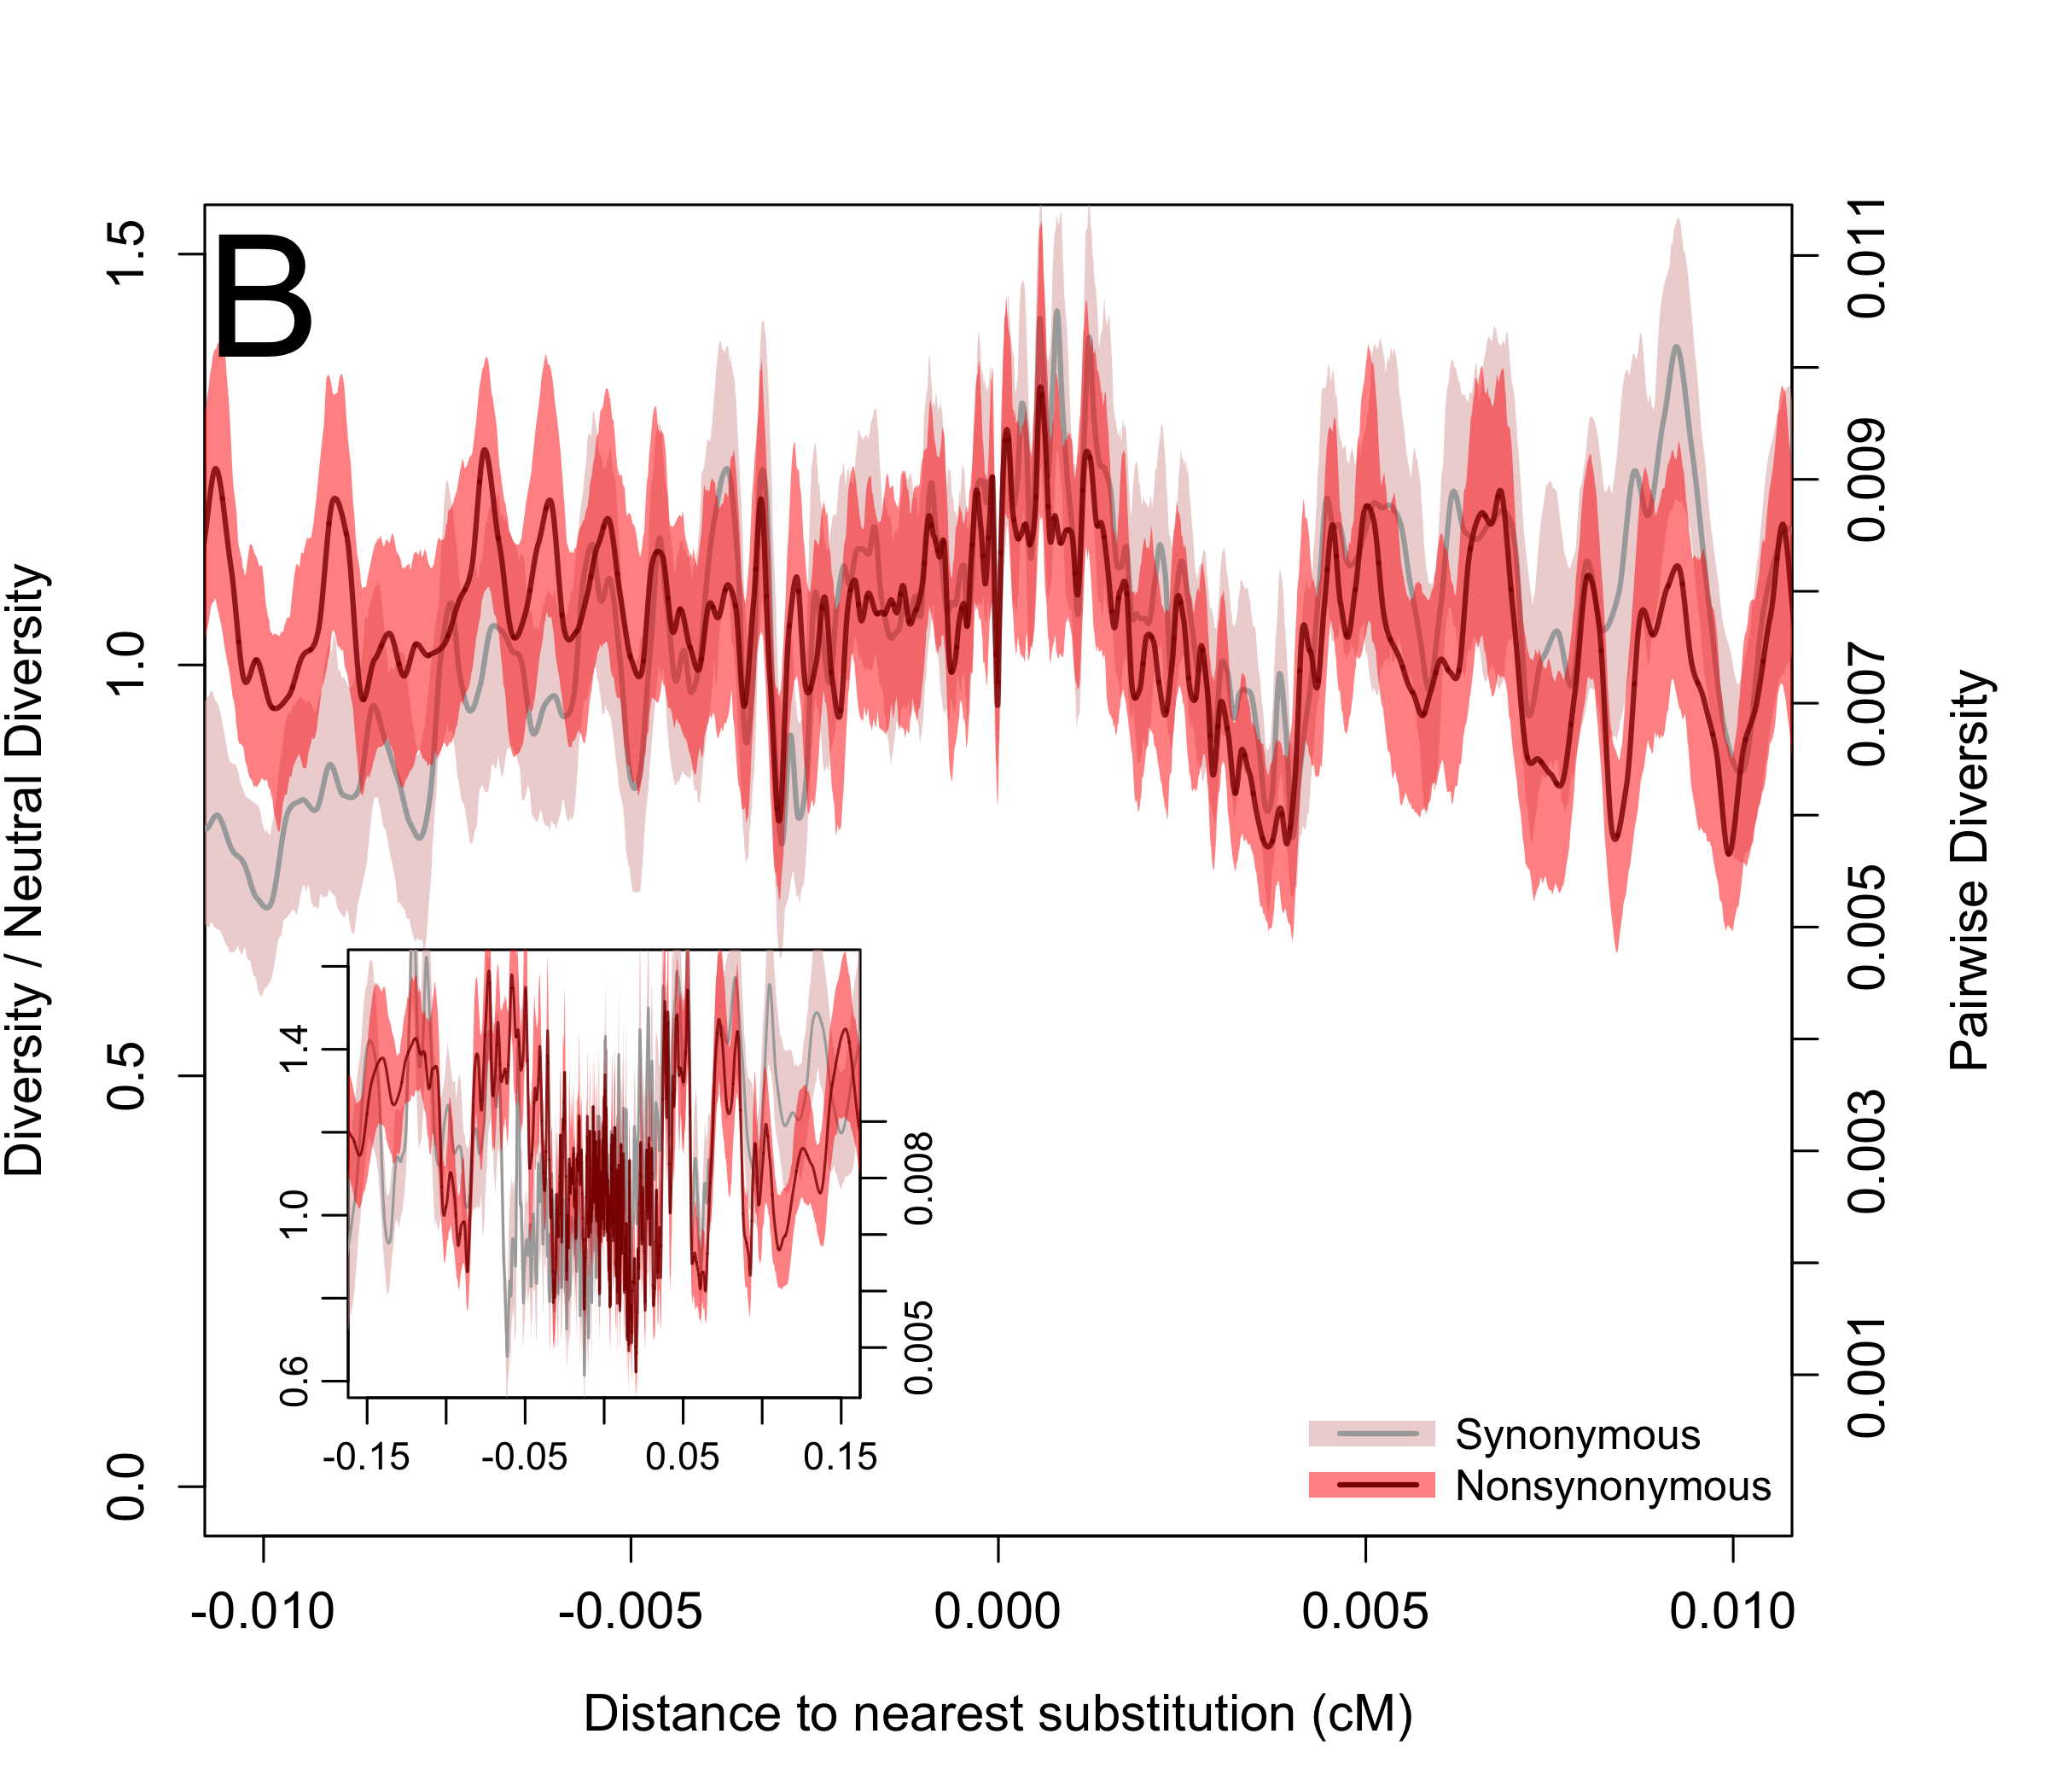
\includegraphics[width=.5\textwidth]{FigsAndFiles/plotDiversity_TvM_Unconserved_Significance_June.png}
\caption{ Pairwise diversity surrounding synonymous and nonsynonymous
  substitutions in maize at highly conserved (A) or unconserved (B) sites.  Bootstrap-based 95\% confidence intervals are depicted via shading. Inset plots depict a larger range on the x-axis. \label{sFig:consUncons}}
\end{figure}
\clearpage

\begin{figure}
  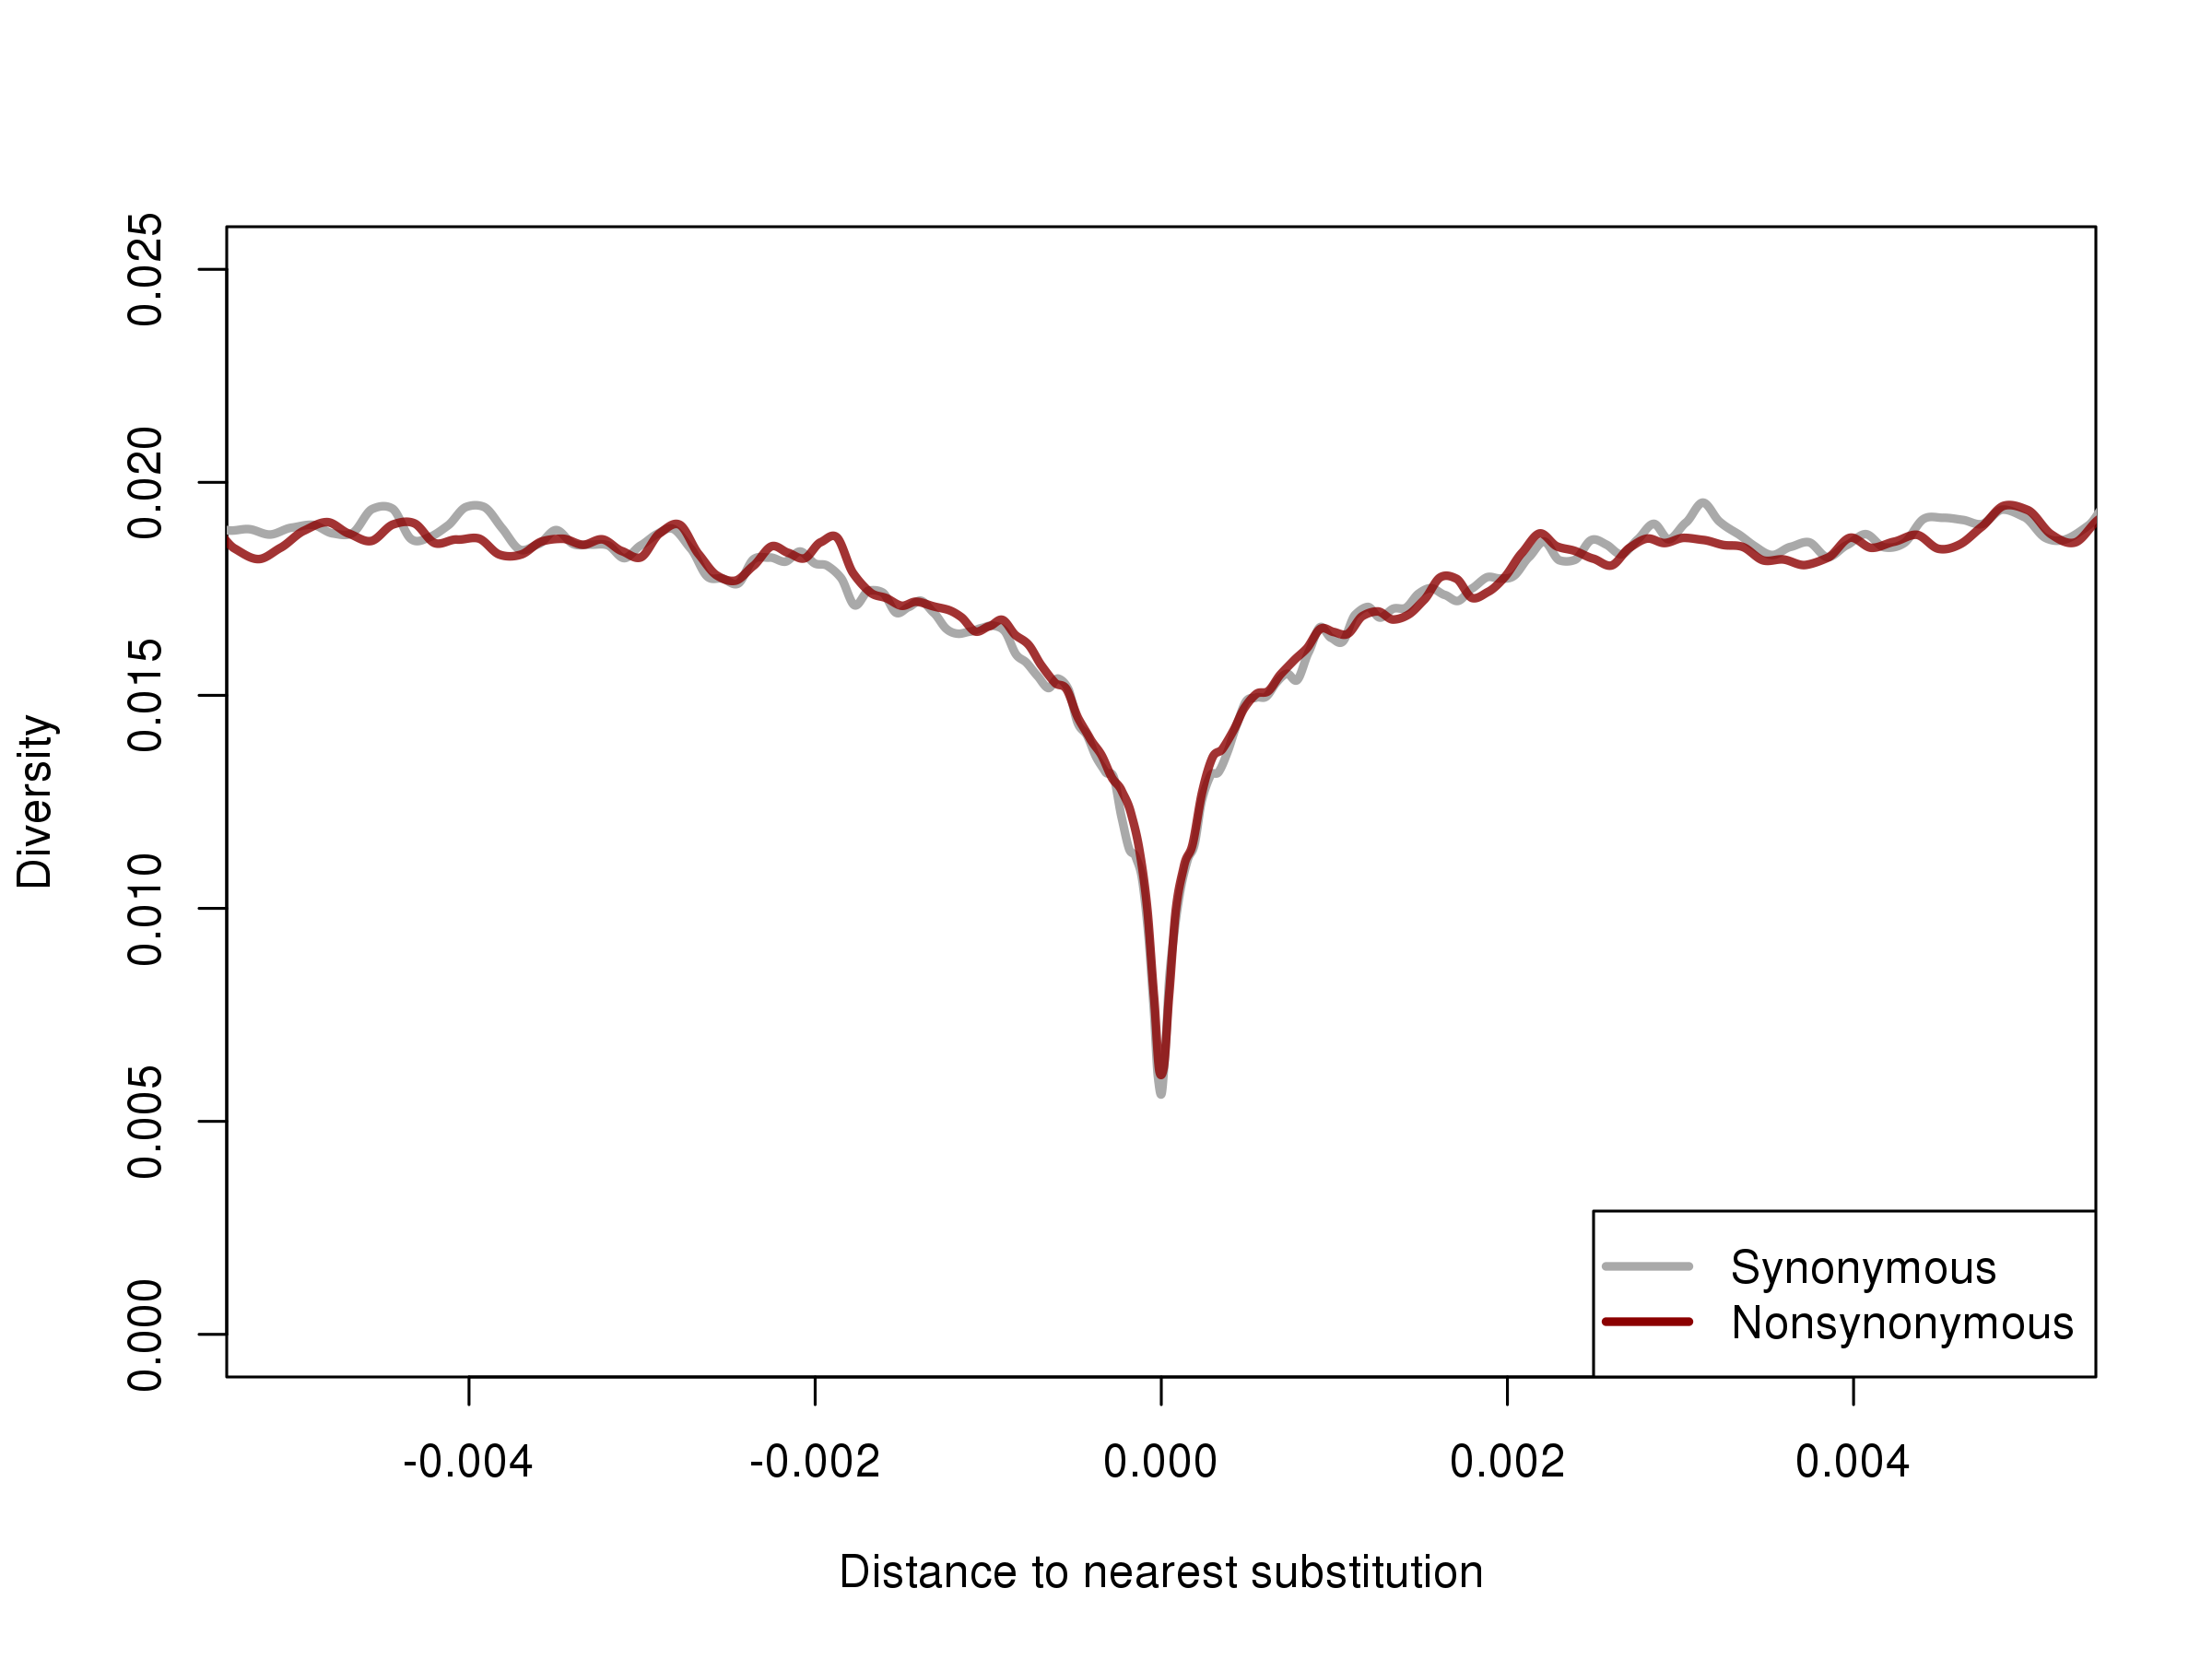
\includegraphics[width=\textwidth]{FigsAndFiles/plotDiversity_TvM_Singletons.png}
\caption{ Singleton diversity surrounding synonymous and nonsynonymous
  substitutions in maize. \label{sFig:singleton}}
\end{figure}
\clearpage


\begin{figure}
  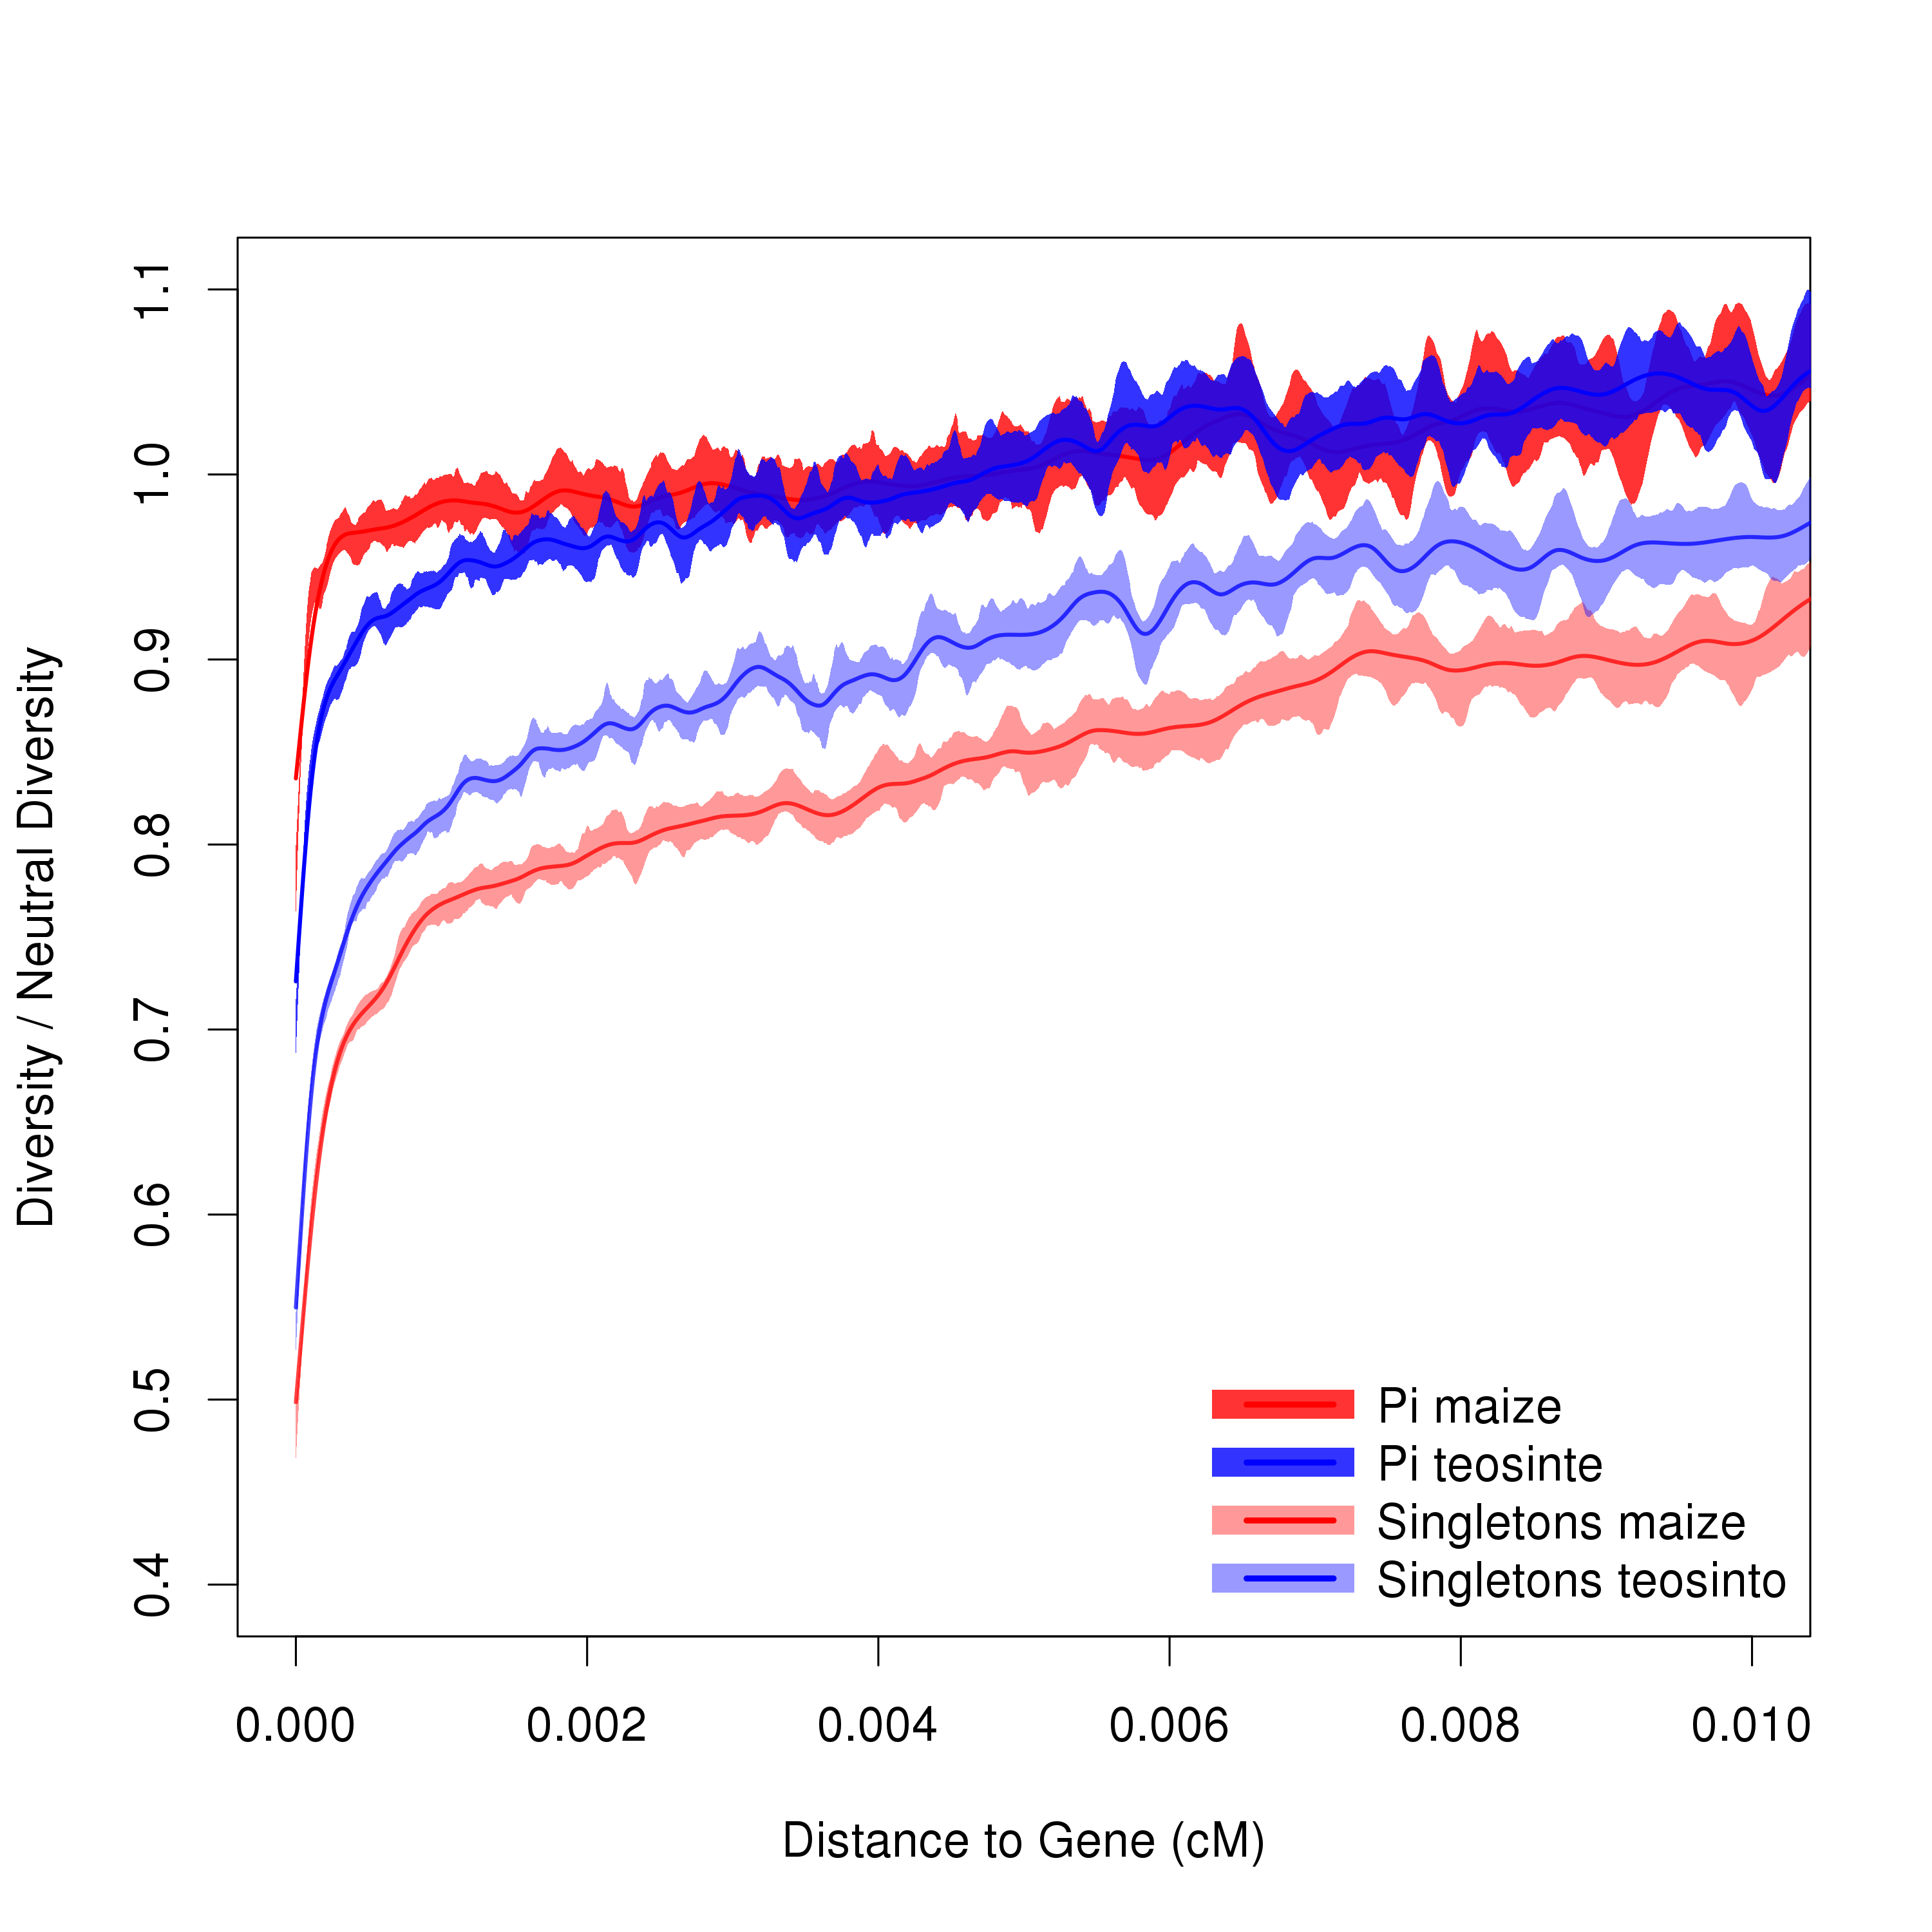
\includegraphics[width=\textwidth]{FigsAndFiles/distanceToGene_WithSignificance_Folded2_maizeAndTeoSingleVsPi.png}
\caption{ Relative diversity versus distance to nearest gene in maize and teosinte. Relative diversity is calculated by comparing to the mean diversity in all windows $\geq 0.02 cM$ from the nearest gene. Lines depict cubic smoothing splines with smoothing parameters chosen via generalized cross validation and shading depicts bootstrap-based 95\% confidence intervals.  \label{sFig:singletonPi}}
\end{figure}
\clearpage


\begin{figure}
  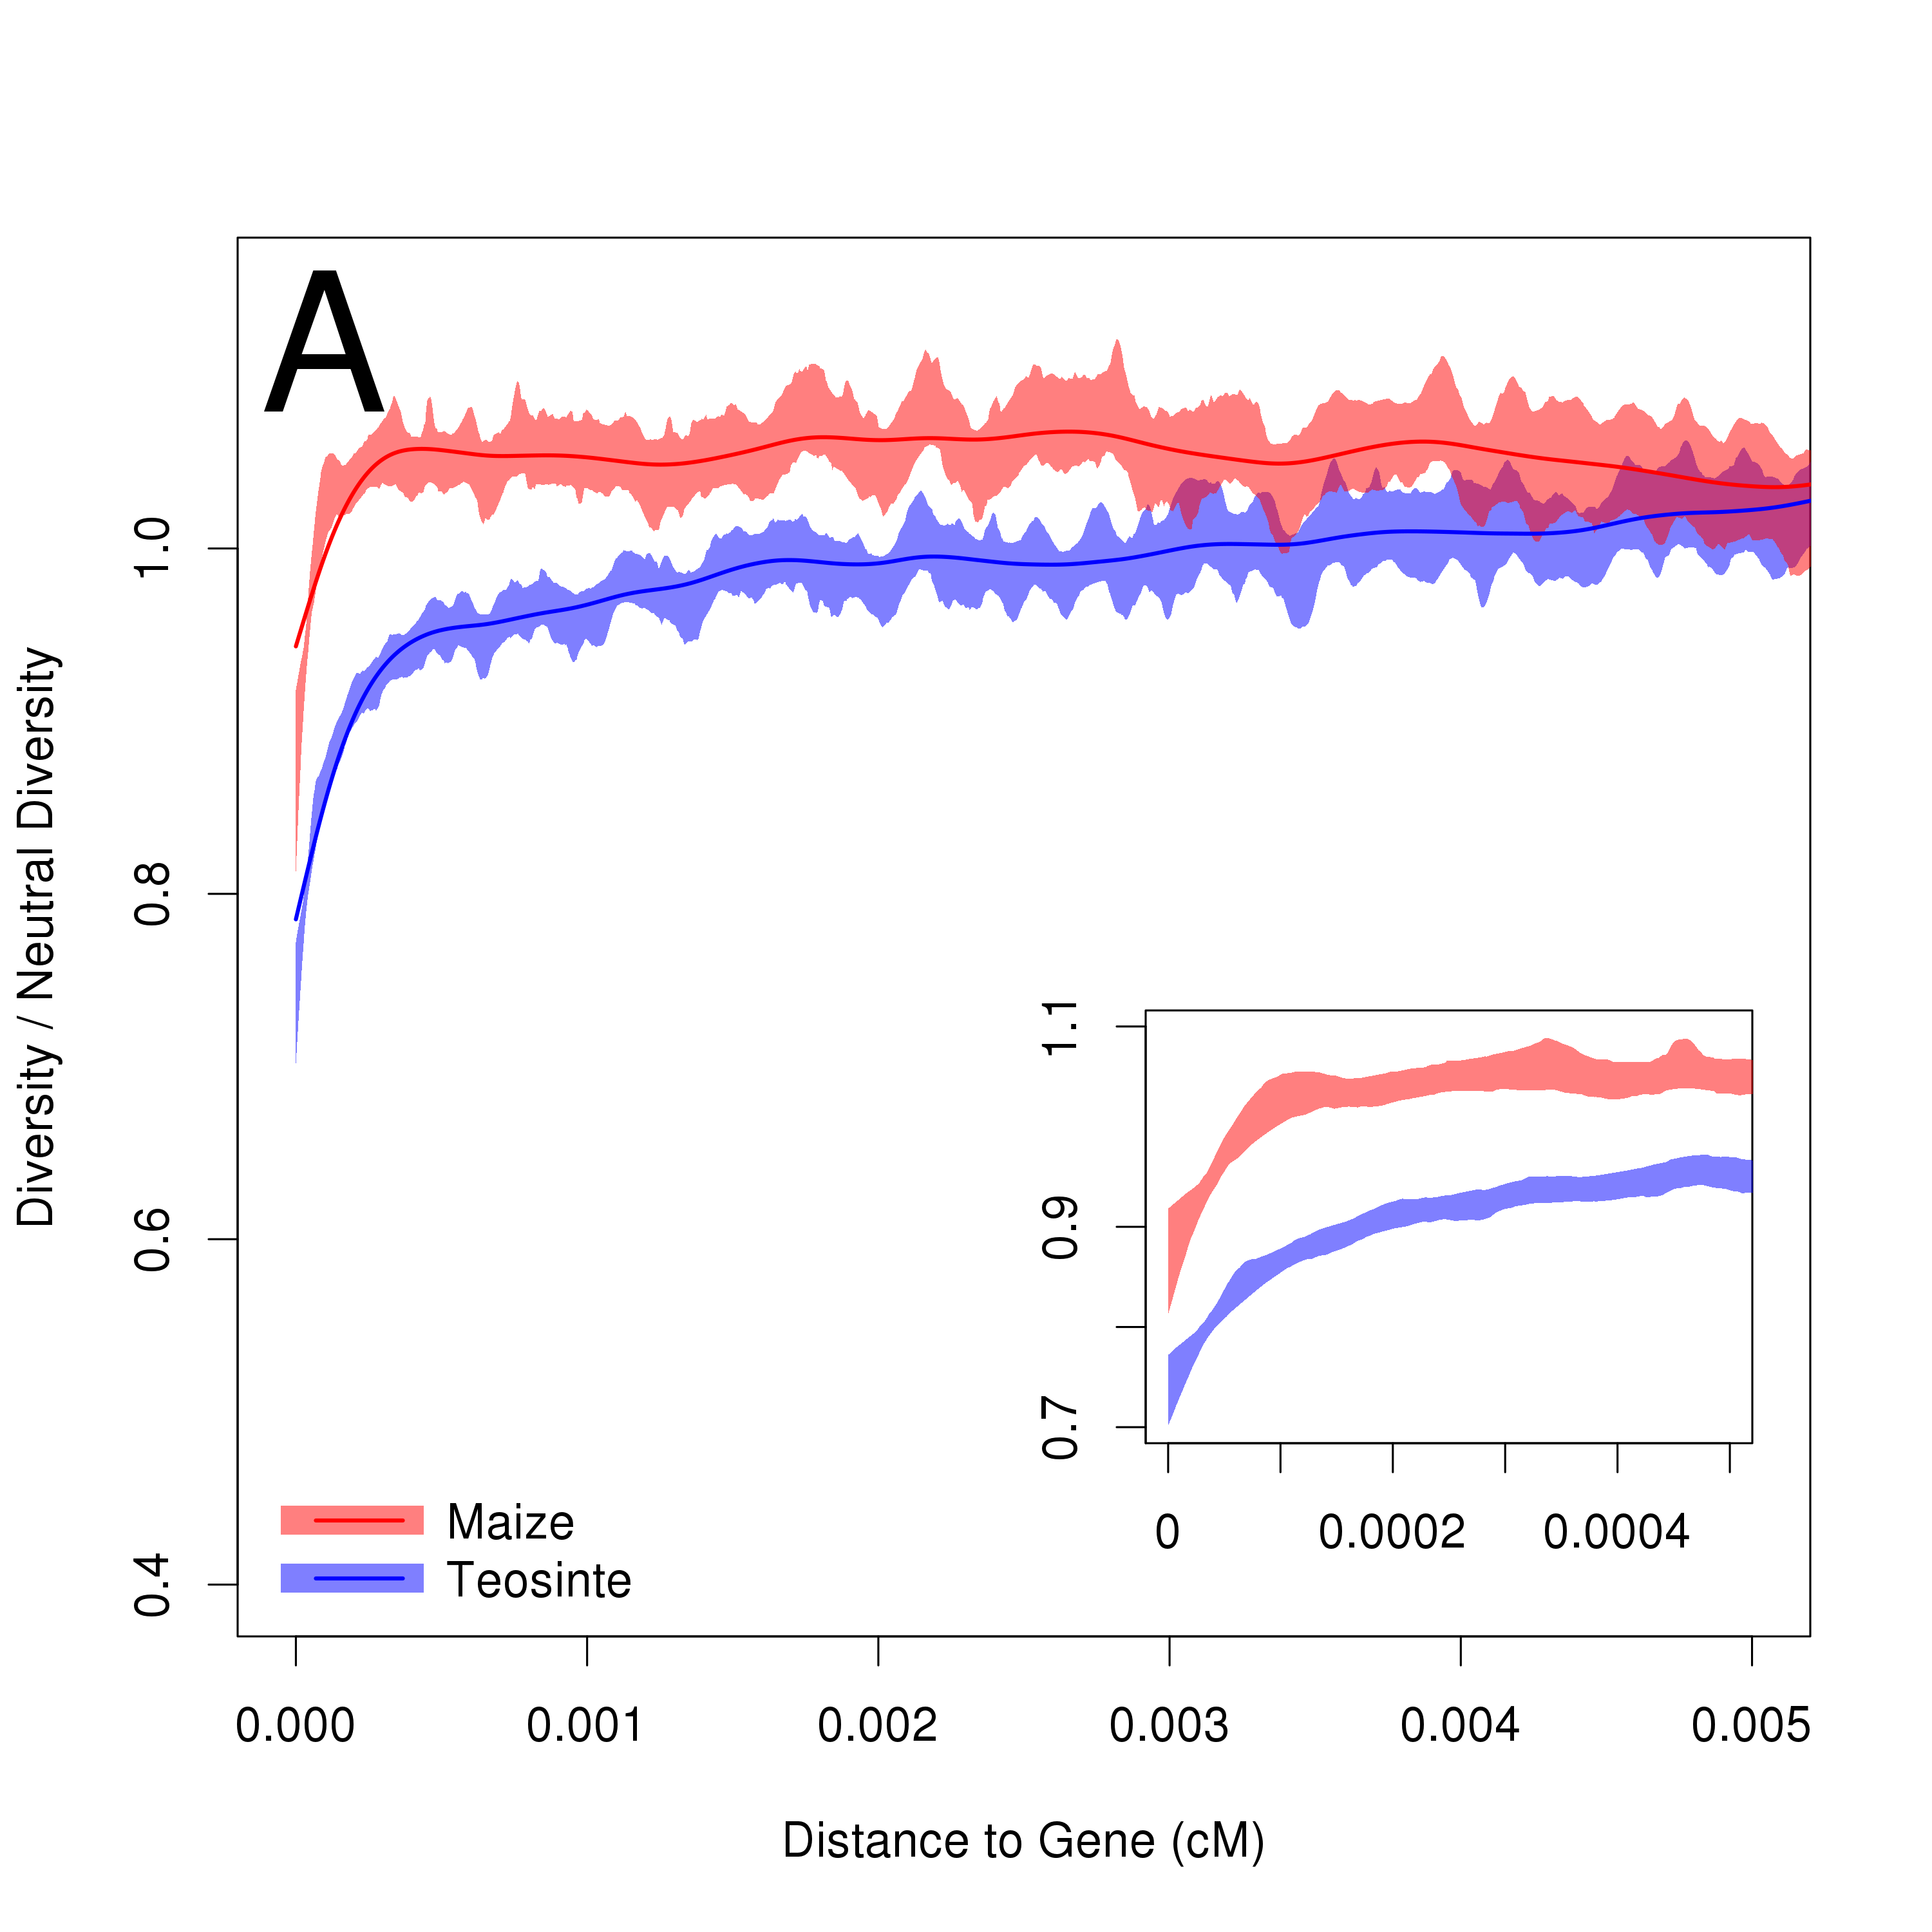
\includegraphics[width=.5\textwidth]{FigsAndFiles/distanceToGene_Unselected_manuscript.png}
    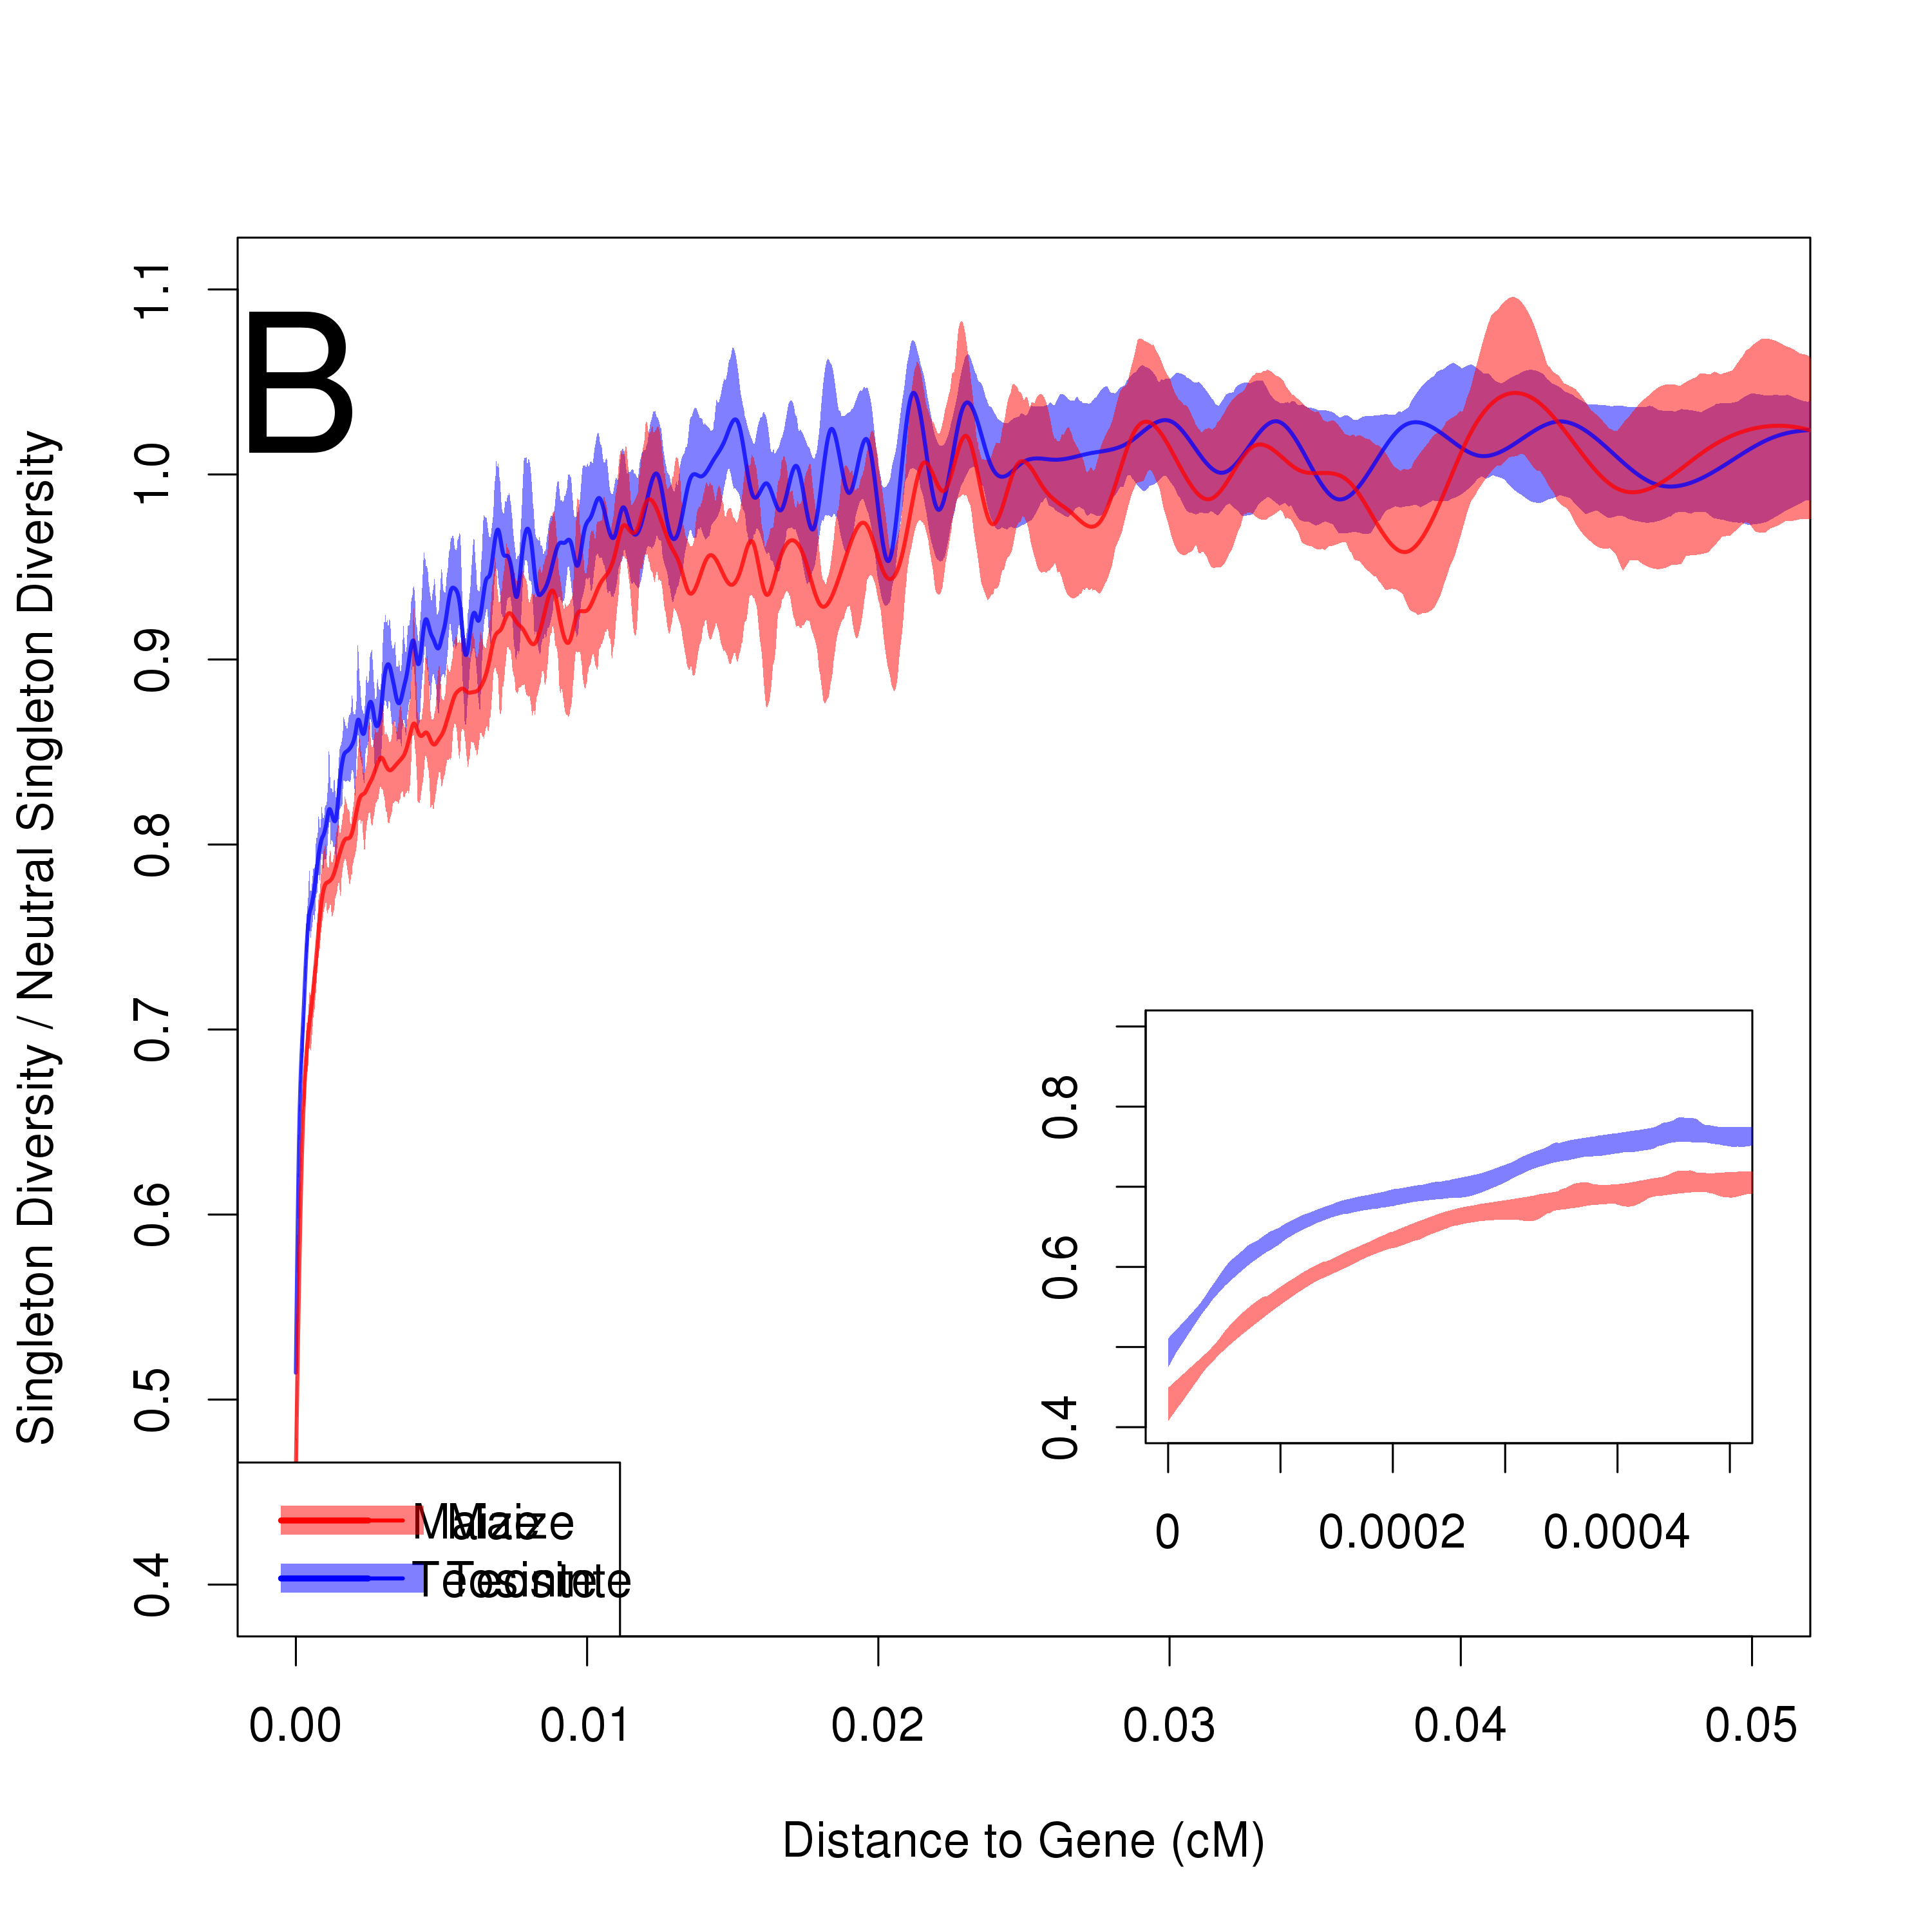
\includegraphics[width=.5\textwidth]{FigsAndFiles/distanceToGene_unselected_Singletons_manuscript.png}
\caption{ Relative level of diversity versus distance to the nearest gene, in maize and teosinte, based on only sites that do not show evidence of hard or soft sweeps according to H12. Two measures of diversity were investigated. {\bf A} displays pairwise diversity,
which is most influenced by intermediate frequency alleles and therefore depicts more ancient evolutionary patterns, and {\bf B} depicts singleton diversity, influenced by rare alleles and thus depicting evolutionary patterns in the recent past. Bootstrap-based 95\% confidence intervals are depicted via shading. Inset plots depict a smaller range on the x-axis. \label{sFig:H12}}
\end{figure}
\clearpage


\begin{figure}
  \begin{center}
  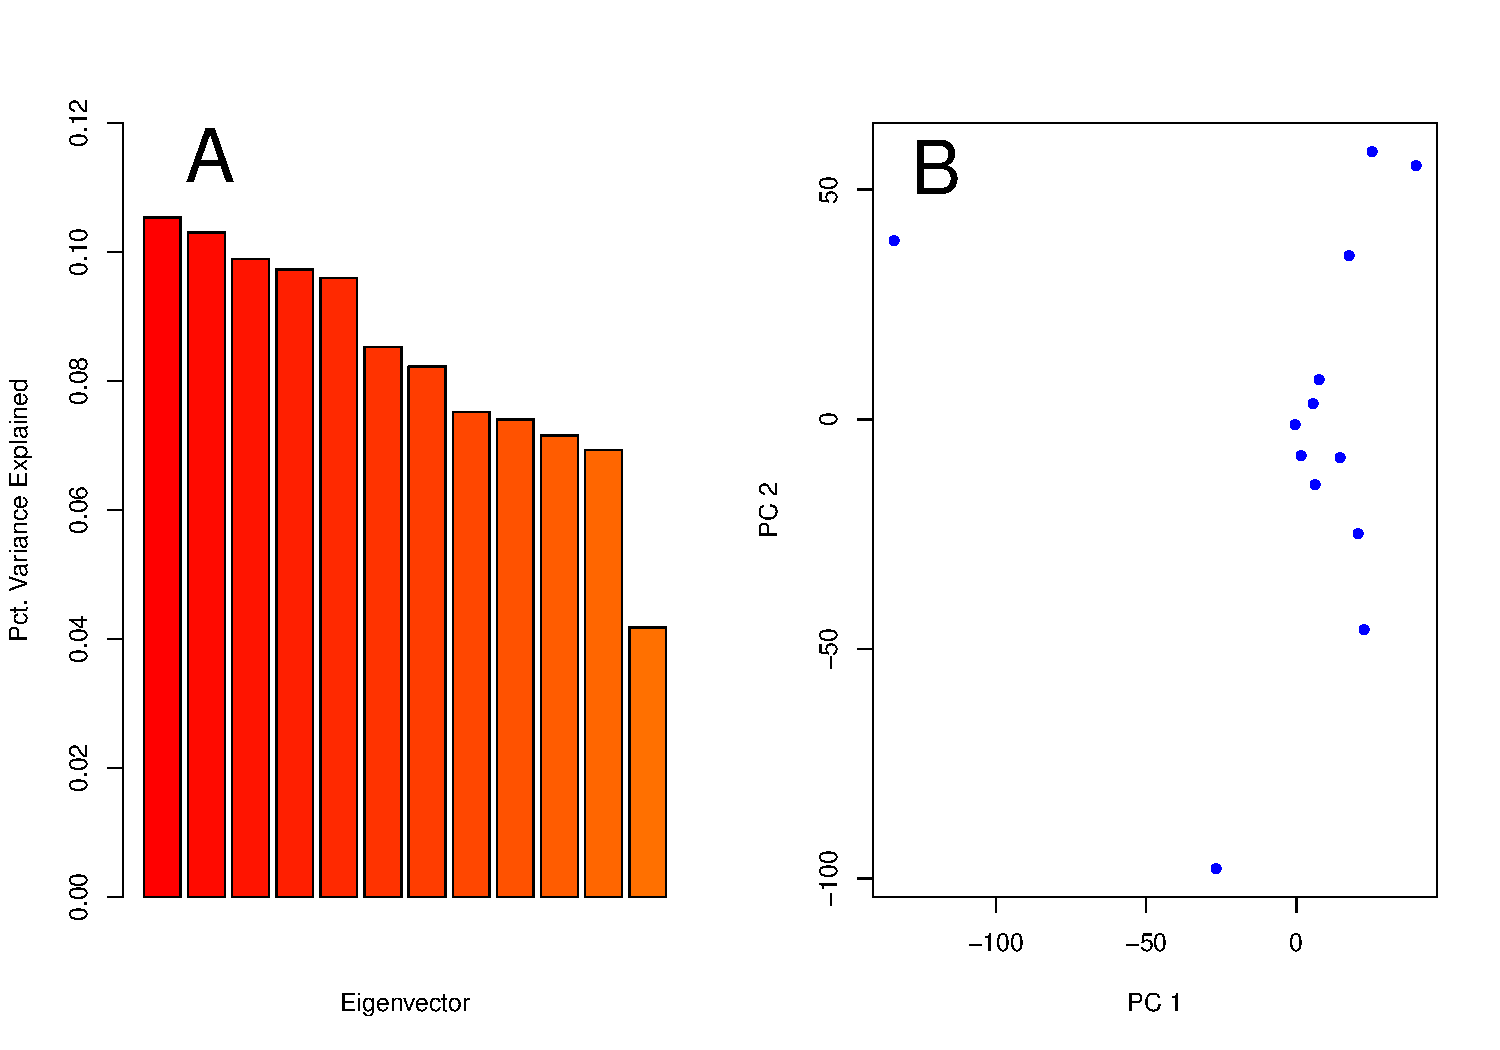
\includegraphics[width=.75\textwidth]{FigsAndFiles/tilPCA_aug.pdf}\\
  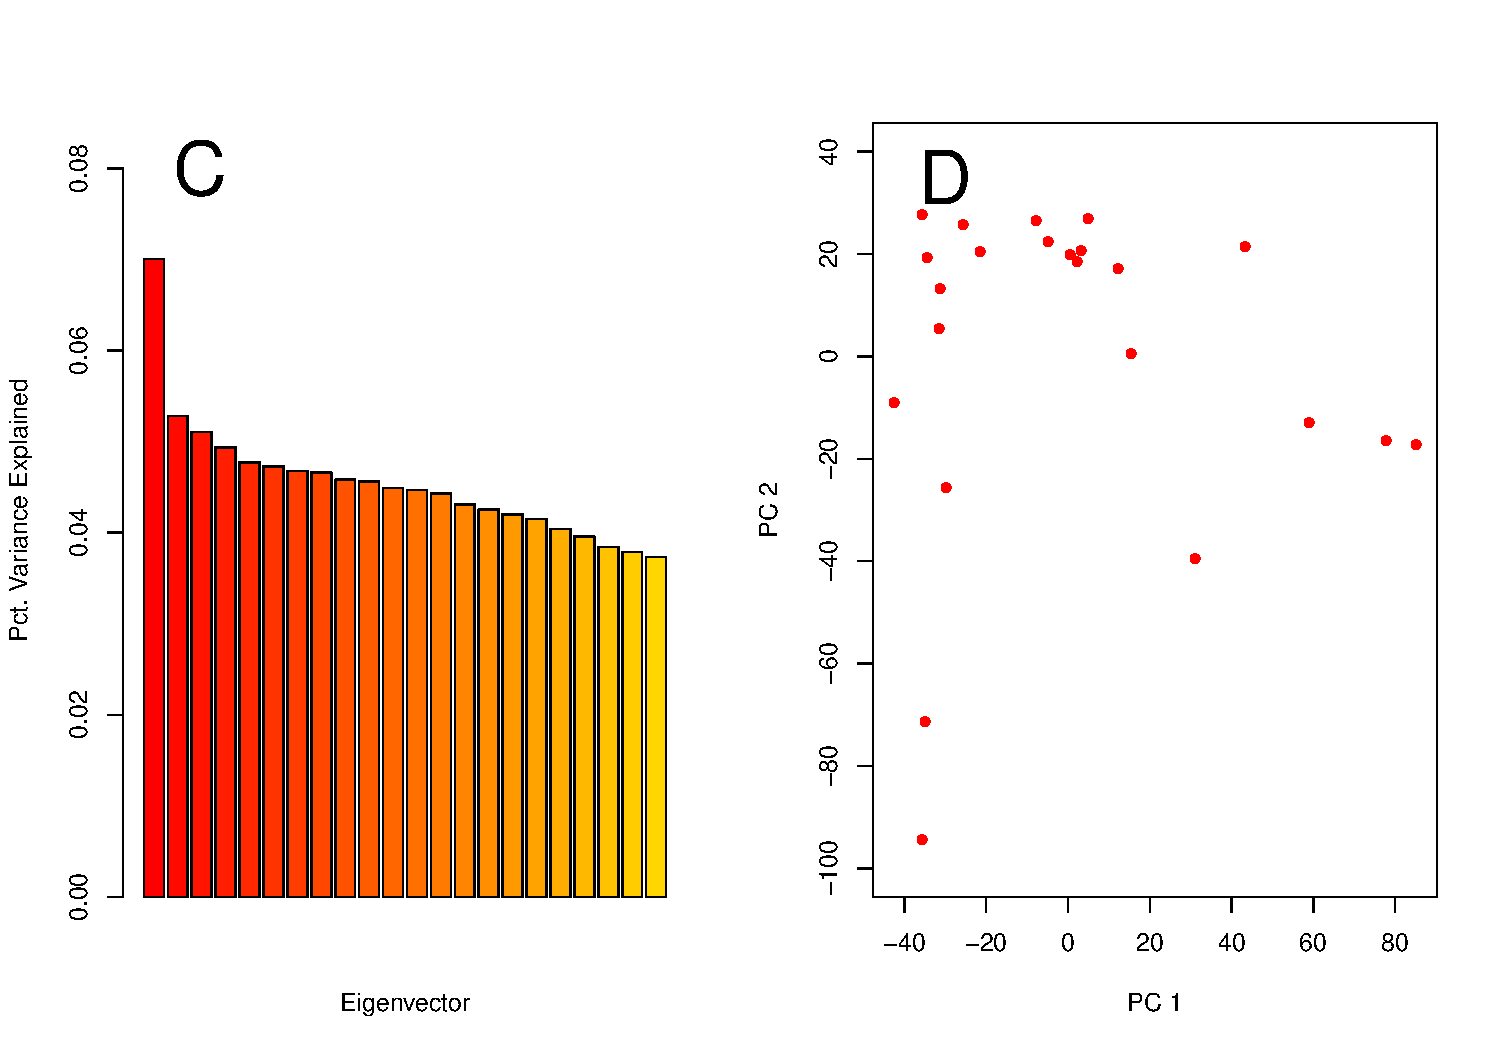
\includegraphics[width=.75\textwidth]{FigsAndFiles/bknPCA_aug.pdf}\\
  \end{center}
  \caption{Principal component analysis of teosinte and maize individuals to ensure that no close relatives were inadvertantly included in our study. Plots are based on a random sample of 10,000 SNPs. {\bf A:} Percentage of total variance explained by each principal component for teosinte. {\bf B:} PC1 vs PC2 for all 13 teosinte individuals. {\bf C:} Percentage of total variance explained by each principal component for maize. {\bf D:} PC1 vs PC2 for all 23 maize individuals. \label{sFig:PCA}}
\end{figure}
\clearpage


\begin{figure}
%  \begin{center}
  \begin{tabular}{c|c}
    \bf Maize & \bf Teosinte \\ \hline \hline
    BKN009 &  TIL01 \\
    BKN010 & TIL02 \\
    BKN011 & TIL03 \\
    BKN014 & TIL04-TIP454 \\
    BKN015 & TIL07 \\
    BKN016 & TIL09 \\
    BKN017 & TIL10 \\
    BKN018 & TIL11 \\
    BKN019 & TIL12 \\
    BKN020 & TIL14-TIP498 \\
    BKN022 & TIL15 \\
    BKN023 & TIL16 \\
    BKN025 & TIL17 \\
    BKN026 & \\
    BKN027 & \\
    BKN029 & \\
    BKN030 & \\
    BKN031 & \\
    BKN032 & \\
    BKN033 & \\
    BKN034 & \\
    BKN035 & \\
    BKN040 & \\
  \end{tabular} 
%  \end{center}
  \caption{ A list of maize and teosinte individuals included in this study. Sequencing and details were previously described by \jri{cite chia and lemmon}   \label{sTab:list} }
\end{figure}
\clearpage

\begin{figure}
  \def\arraystretch{2}
%  \begin{center}
  \begin{tabular}{l|c|c|c}
    \bf Parameter & \bf Initial value & \bf Upper bound & \bf Lower bound\\ \hline 
    $\frac{N_b}{N_a}$ & 0.02 & $1\times10^{-7}$ & 2 \\ 
    $\frac{N_{m}}{N_a}$ & 3 & $1\times10^{-7}$ & 200 \\
    $\frac{T_b}{2N_a}$ & 0.04 & 0  & 1 \\ 
    $\frac{M_{mt}}{N_a}$ & $1\times10^{-10}$ & $1\times10^{-7}$ & 0.001 \\
    $\frac{M_{tm}}{N_a}$ & $1\times10^{-10}$ & $1\times10^{-7}$ & 0.001 \\
  \end{tabular} 
%  \end{center}
  \caption{ Parameters, initial values, and boundaries used for model-fitting with $\delta\alpha\delta{i}$. Parameters are shown in the units utilized by $\delta\alpha\delta{i}$, although in the text simplified units are reported.   \label{sTab:dadi} }
    \def\arraystretch{1} % undo stretching
\end{figure}
\clearpage
 
%\nocite{*}


\end{article}
\end{document}
